\documentclass{beamer}
% Class options include: notes, handout, trans
%                        
\usepackage[finnish]{babel}
% Theme for beamer presentation.
\usepackage{beamerthemesplit,xmpmulti,cancel} 

% Other themes include: beamerthemebars, beamerthemelined,beamerthemetree, beamerthemeplain
\usepackage[utf8]{inputenc}
\usefonttheme{professionalfonts}

\title[Aalto-yliopiston perustieteiden korkeakoulu]{Kysyntäohjautuvan joukkoliikenteen matemaattisia malleja ja algoritmeja}
%\subtitle{Examples of lists, columns and graphics}    % Enter your title between curly braces
\author[L. Häme]{Lauri Häme}                 % Enter your name between curly braces
\institute[Aalto-yliopiston perustieteiden korkeakoulu]{Aalto-yliopiston perustieteiden korkeakoulu}      % Enter your institute name between curly braces
\date{\today}      % Enter the date or \today between curly braces

\usepackage{graphicx}

    \setbeamerfont{section title}{parent=title}
    \setbeamercolor{section title}{parent=titlelike}
    \defbeamertemplate*{section pages}{default}[1][]
    {
      \centering
        \begin{beamercolorbox}[sep=8pt,center,#1]{section title}
          \usebeamerfont{section title}\insertsection\par
        \end{beamercolorbox}
    }
    \newcommand*{\secpage}{\usebeamertemplate*{section pages}}
    
\begin{document}

% Creates title page of slide show using above information
\begin{frame}
  \titlepage
\end{frame}
%\cancele{Talk for 30 minutes} % Add notes to yourself that will be displayed when typeset with the notes class option.

%\section{Johdanto}
% Creates table of contents slide incorporating all \section and \subsection commands.
%\begin{frame}
%  \tableofcontents
%\end{frame}

%\subsection{Johdanto}
\begin{frame}
  \frametitle{Johdanto}   % Insert frame title between curly braces
  \begin{itemize}
    \item 
Kysyntäohjautuva joukkoliikenne = bussi- ja taksipalvelujen välimuoto, joka perustuu ajoneuvojen joustavaan reititykseen
\begin{itemize}
 \item 
 Matkat tilataan esim. internetistä ja ajoneuvojen reitit muodostuvat reaaliaikaisesti tilausten perusteella
 \end{itemize}
 
  \item 
Väitöskirjassa tarkastellaan kolmea teemaa
 \begin{itemize}
\item
Ajoneuvojen reitinlaskenta
\item
Matkustajien matkansuunnittelu
\item
Taloudellinen tasapaino
\end{itemize}
%  \column{2.5in}
 \end{itemize}

%\framebox{\includegraphics[scale=0.6]{esitys01}}
 
%  \end{columns}
\end{frame}

\section{Reitinlaskenta}
\frame{\secpage}
\subsection{Ongelman määrittely}
\begin{frame}
  \frametitle{Kauppamatkustajan ongelma}   % Insert frame title between curly braces
  \begin{columns}
   \column{2.7in}
  
  \begin{itemize}
    \item 
Tunnetuin reitinlaskentaongelma on ns. kauppamatkustajan ongelma (Traveling Salesman Problem, TSP)
\begin{itemize}
\item
Joukko maantieteellisiä pisteitä, joiden väliset etäisyydet tunnetaan
\item
Tavoitteena on löytää lyhin reitti joka kulkee kaikkien pisteiden kautta
\item
Laskennallisesti haastava ongelma
    \end{itemize}
    \end{itemize}
    \column{2in}
    \centering
 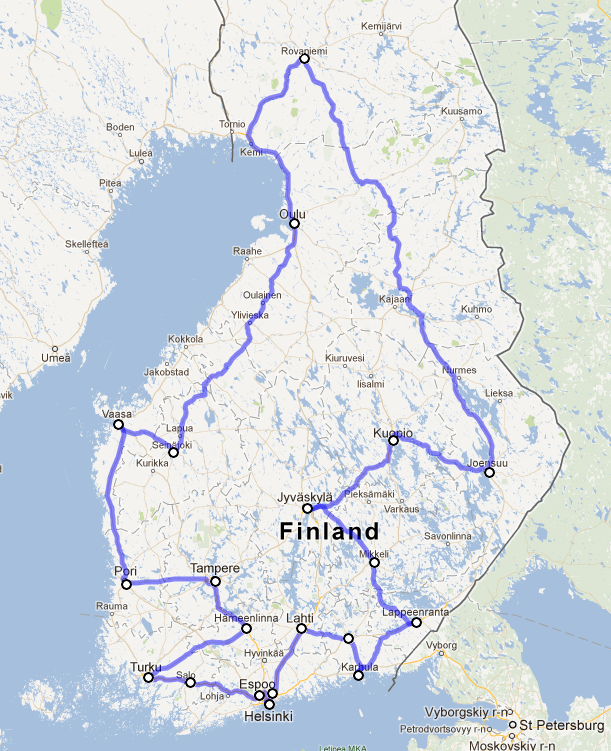
\includegraphics[scale=0.23]{tspdemo03}
    \end{columns}

    \end{frame}

    
%     \begin{frame}
%   \frametitle{Kauppamatkustajan ongelma, esimerkki}   % Insert frame title between curly braces
% \centering
% 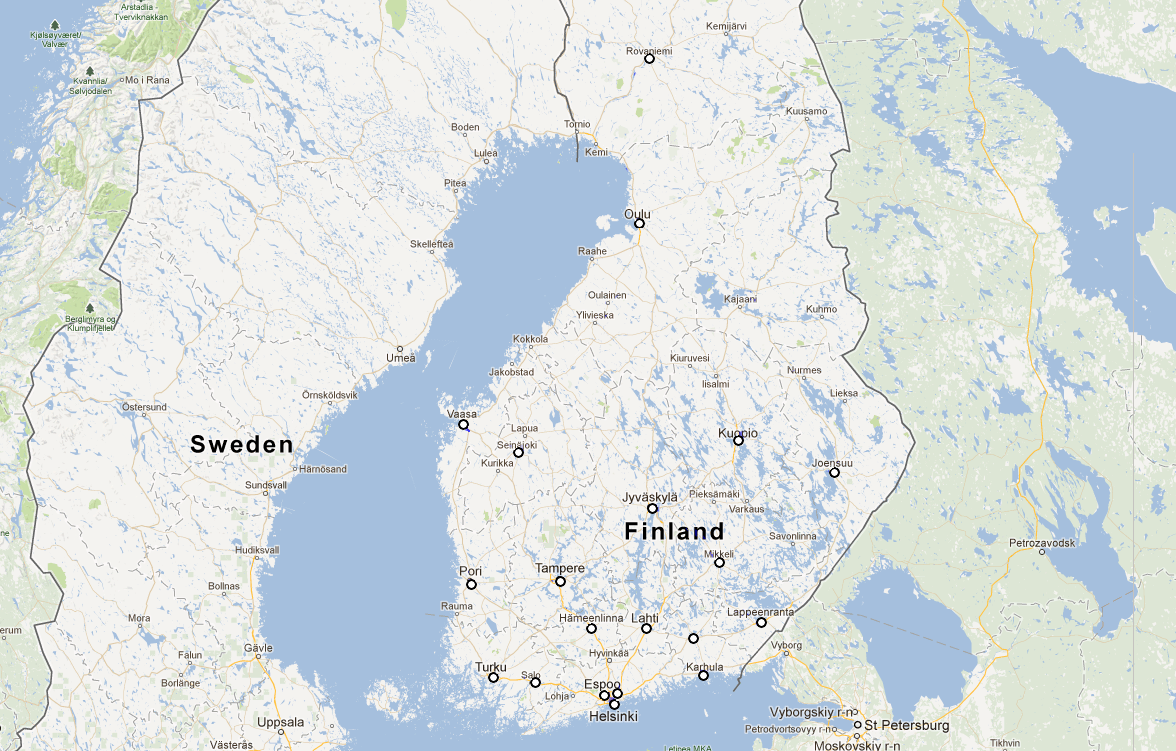
\includegraphics[scale=0.25]{tspdemo01}
%     \end{frame}
%     
%         \begin{frame}
%   \frametitle{Kauppamatkustajan ongelma, esimerkki}   % Insert frame title between curly braces
% \centering
% 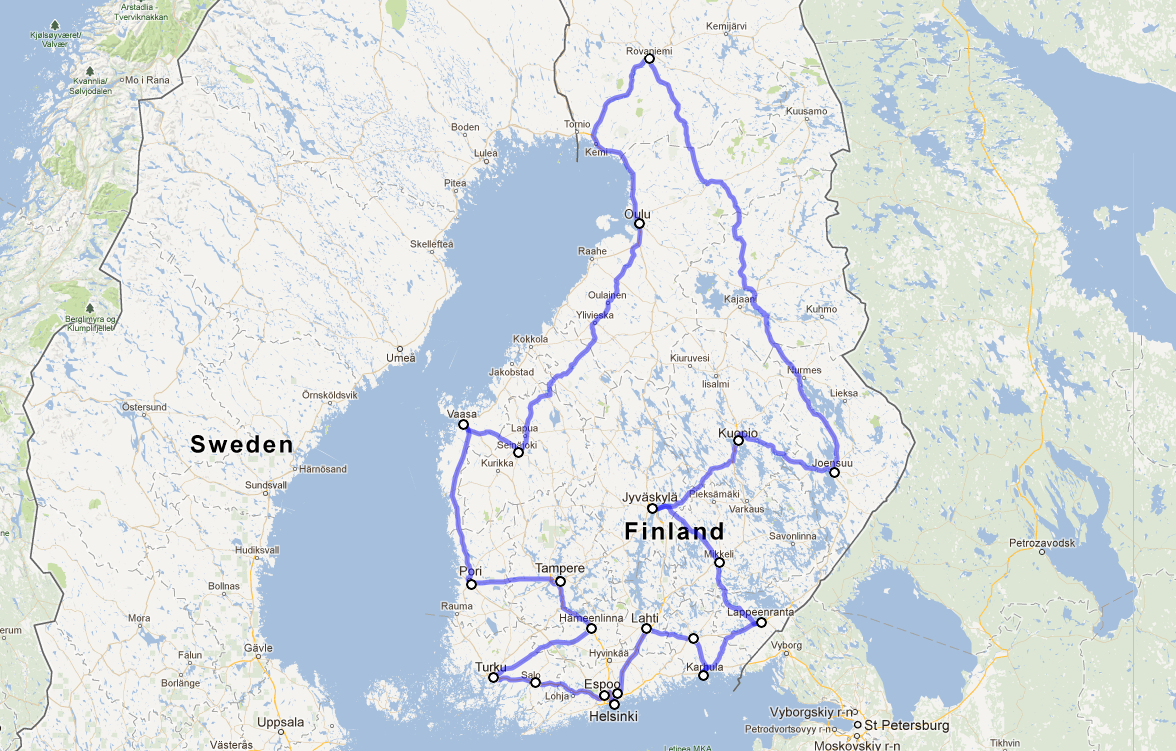
\includegraphics[scale=0.25]{tspdemo02}
%     \end{frame}
%     

%\subsection{Kysyntäohjautuva joukkoliikenne}
\begin{frame}
    \frametitle{Reitinlaskenta kuljetuspalveluissa}
    \begin{itemize}
    \item
    Käytännössä, esim. kuljetuspalveluissa, reitinlaskentaongelma on usein monimutkaisempi
    \item
    Ongelma voi olla staattinen tai dynaaminen
    \item
    Tavoitteita
    \begin{itemize}
     \item 
     tilausten lukumäärän maksimointi
     \item
     kustannusten minimointi
     \item
     asiakkaiden palvelutason optimointi
    \end{itemize}
    \item
    Rajoituksia
    \begin{itemize}
\item 
Kapasiteetti - Ajoneuvoihin mahtuu vain tietty määrä tavaraa/ matkustajia kerrallaan
\item
Aika - Kuljetus ei saa kestää liian kauan
\item
Edeltävyys - Esim. noutopisteessä pitää käydä ennen toimituspistettä
\end{itemize}
% \item
% Ajoneuvoja eli laskettavia reittejä voi olla useita
% \begin{itemize}
%  \item 
%  Ajoneuvojen ja matkustajien yhdistely
% \end{itemize}
  \end{itemize}

\end{frame}




\begin{frame}
  \frametitle{Reitinlaskenta kysyntäohjautuvassa joukkoliikenteessä}   % Insert frame title between curly braces
  \begin{columns}[c]
  \column{3.5in}  % slides are 3in high by 5in wide
  \begin{itemize}
    %\item 
    %Kysyntäohjautuva joukkoliikenne perustuu pienten tai keskisuurten ajoneuvojen (esim. minibussien) joustavaan reititykseen 
    \item
    Asiakkaat voivat tilata matkoja reaaliaikaisesti esim. internet-käyttöliittymällä
    \item
    Ajoneuvojen reitit muodostuvat tilattujen matkojen perusteella
 %\item 
 %Jokaiselle uudelle asiakkaalle valitaan ajoneuvo ja valitulle ajoneuvolle määrätään uusi reitti
  \item
 Ajoneuvon ja reitin valinnassa pitää ottaa huomioon mm.
 \begin{itemize}
  \item 
  Uuden asiakkaan aiheuttama reitin pitenemä
  \item
  Uuden asiakkaan palvelutaso ja muille asiakkaille aiheutuva palvelutason muutos
  \item
  Kysyntäennuste
 \end{itemize}

  \end{itemize}
    \column{1.5in}
\centering

%\framebox{
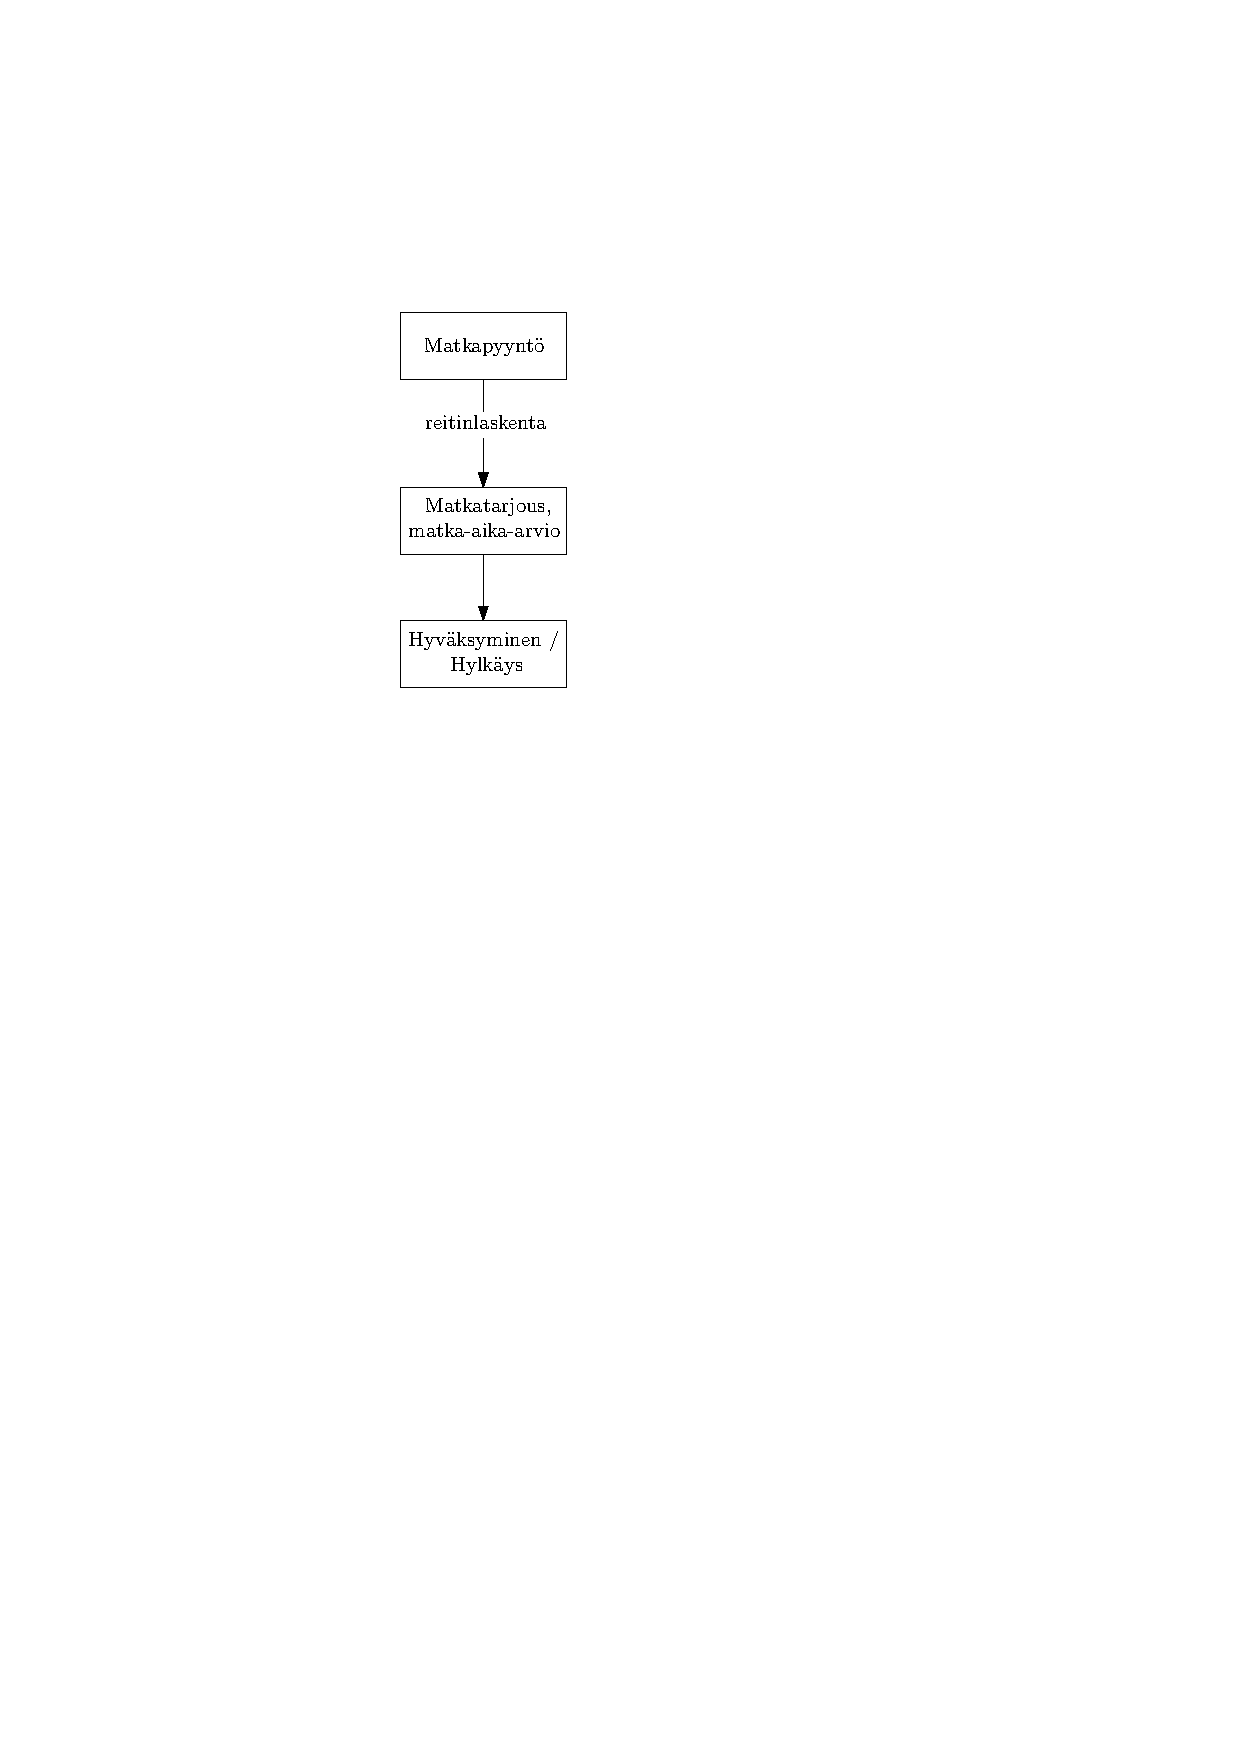
\includegraphics[scale=0.8]{tilauskaavio02}
%}
 
  \end{columns}
\end{frame}

%         \begin{frame}
%   \frametitle{Kysyntäohjautuva joukkoliikenne, 1 ajoneuvo, esimerkki }   % Insert frame title between curly braces
% \begin{center}
% 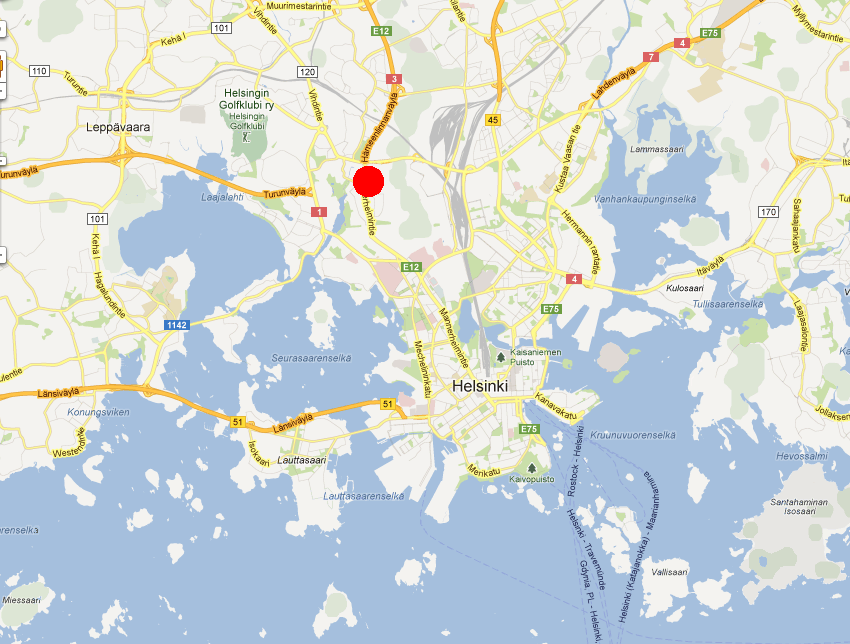
\includegraphics[scale=0.3]{ekademo01}
% \end{center}
% \end{frame}
% 
%         \begin{frame}
%   \frametitle{Kysyntäohjautuva joukkoliikenne, 1 ajoneuvo, esimerkki}   % Insert frame title between curly braces
% \begin{center}
% 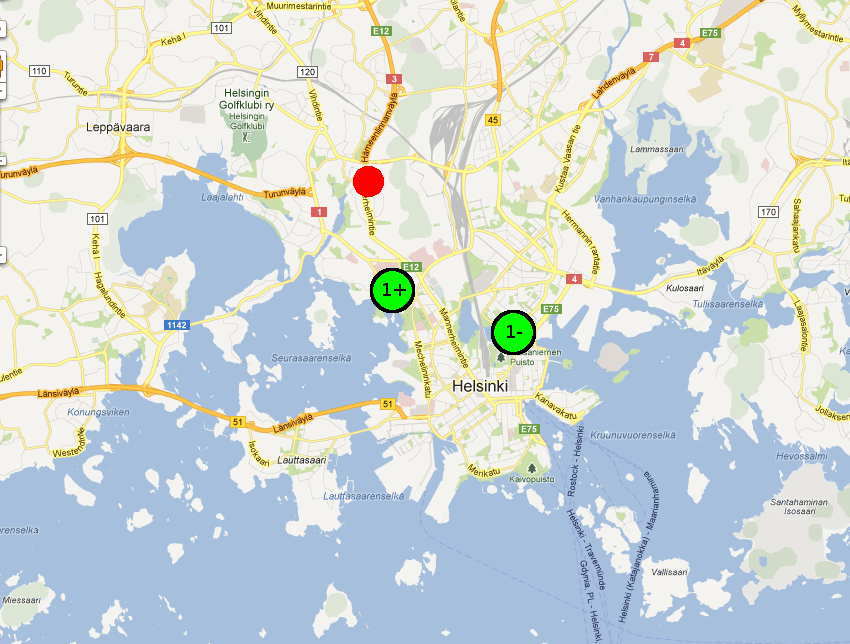
\includegraphics[scale=0.3]{ekademo02}
% \end{center}
%     \end{frame}
%     
%             \begin{frame}
%   \frametitle{Kysyntäohjautuva joukkoliikenne, 1 ajoneuvo, esimerkki}   % Insert frame title between curly braces
% \begin{center}
% 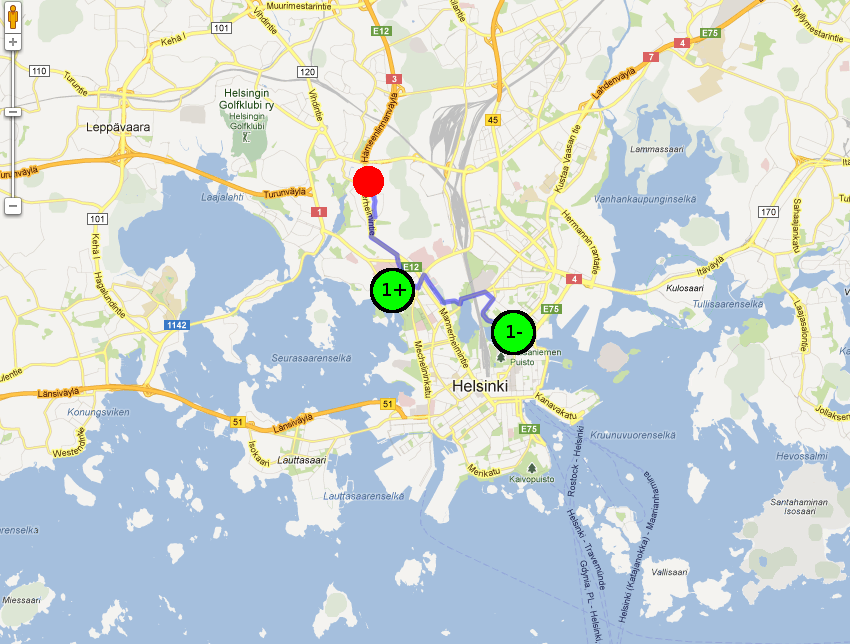
\includegraphics[scale=0.3]{ekademo03}
% \end{center}
%     \end{frame}
%     
%             \begin{frame}
%   \frametitle{Kysyntäohjautuva joukkoliikenne, 1 ajoneuvo, esimerkki}   % Insert frame title between curly braces
% \begin{center}
% 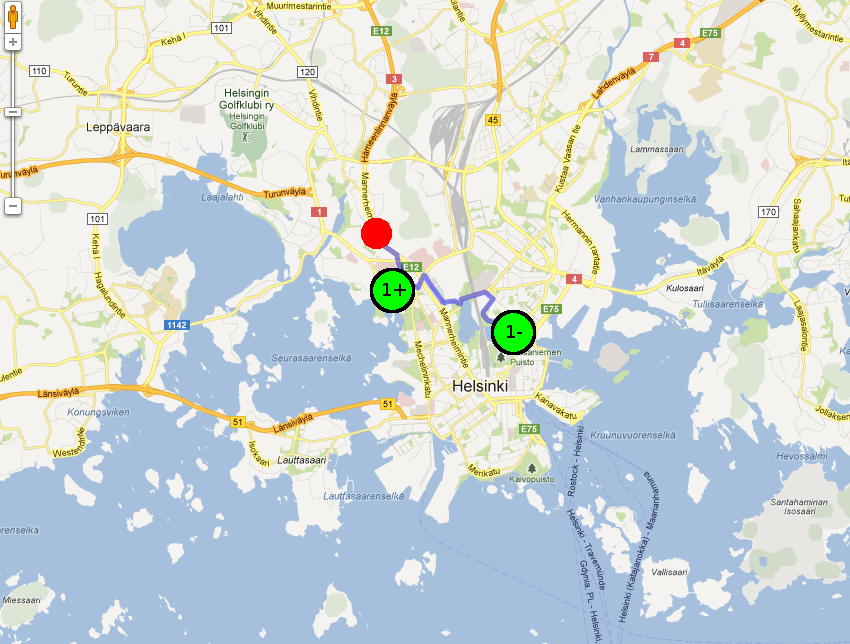
\includegraphics[scale=0.3]{ekademo04}
% \end{center}
%     \end{frame}
%     
%             \begin{frame}
%   \frametitle{Kysyntäohjautuva joukkoliikenne, 1 ajoneuvo, esimerkki}   % Insert frame title between curly braces
% \begin{center}
% 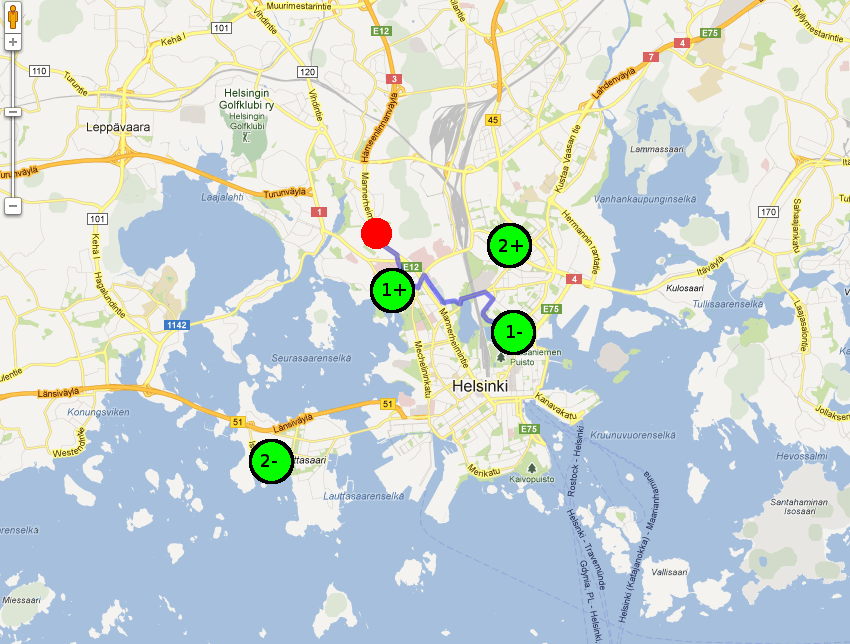
\includegraphics[scale=0.3]{ekademo05}
% \end{center}
%     \end{frame}
%     
%             \begin{frame}
%   \frametitle{Kysyntäohjautuva joukkoliikenne, 1 ajoneuvo, esimerkki}   % Insert frame title between curly braces
% \begin{center}
% 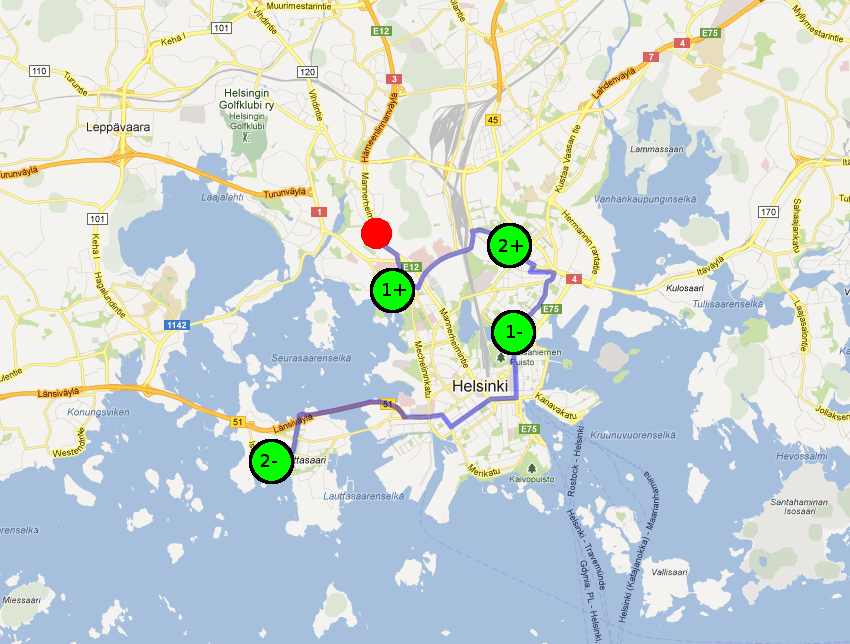
\includegraphics[scale=0.3]{ekademo06}
% \end{center}
%     \end{frame}

%     
% \begin{frame}
% \frametitle{Aikarajoitteet}
% \begin{itemize}
%  \item 
%  Matka-aika voi pidentyä yllättäen reittimuutosten johdosta
%  \item
%  Palvelutasosta voidaan huolehtia aikarajoitteilla
%  \begin{itemize}
%   \item 
%   Esim. lähtö aikaisintaan klo 12:00, perillä viimeistään klo 13:00.
%   %\item 
%   %Aikarajoitteet voivat olla osittain asiakkaan ja osittain järjestelmän määrittämiä
%  \end{itemize}
%  \item
%   Käytetään reitinlaskennassa, jotta tietty minimipalvelutaso toteutuisi
%  \item
%  Liian tiukat rajoitteet vähentävät reitin joustavuutta
% \end{itemize}
% \begin{center}
% 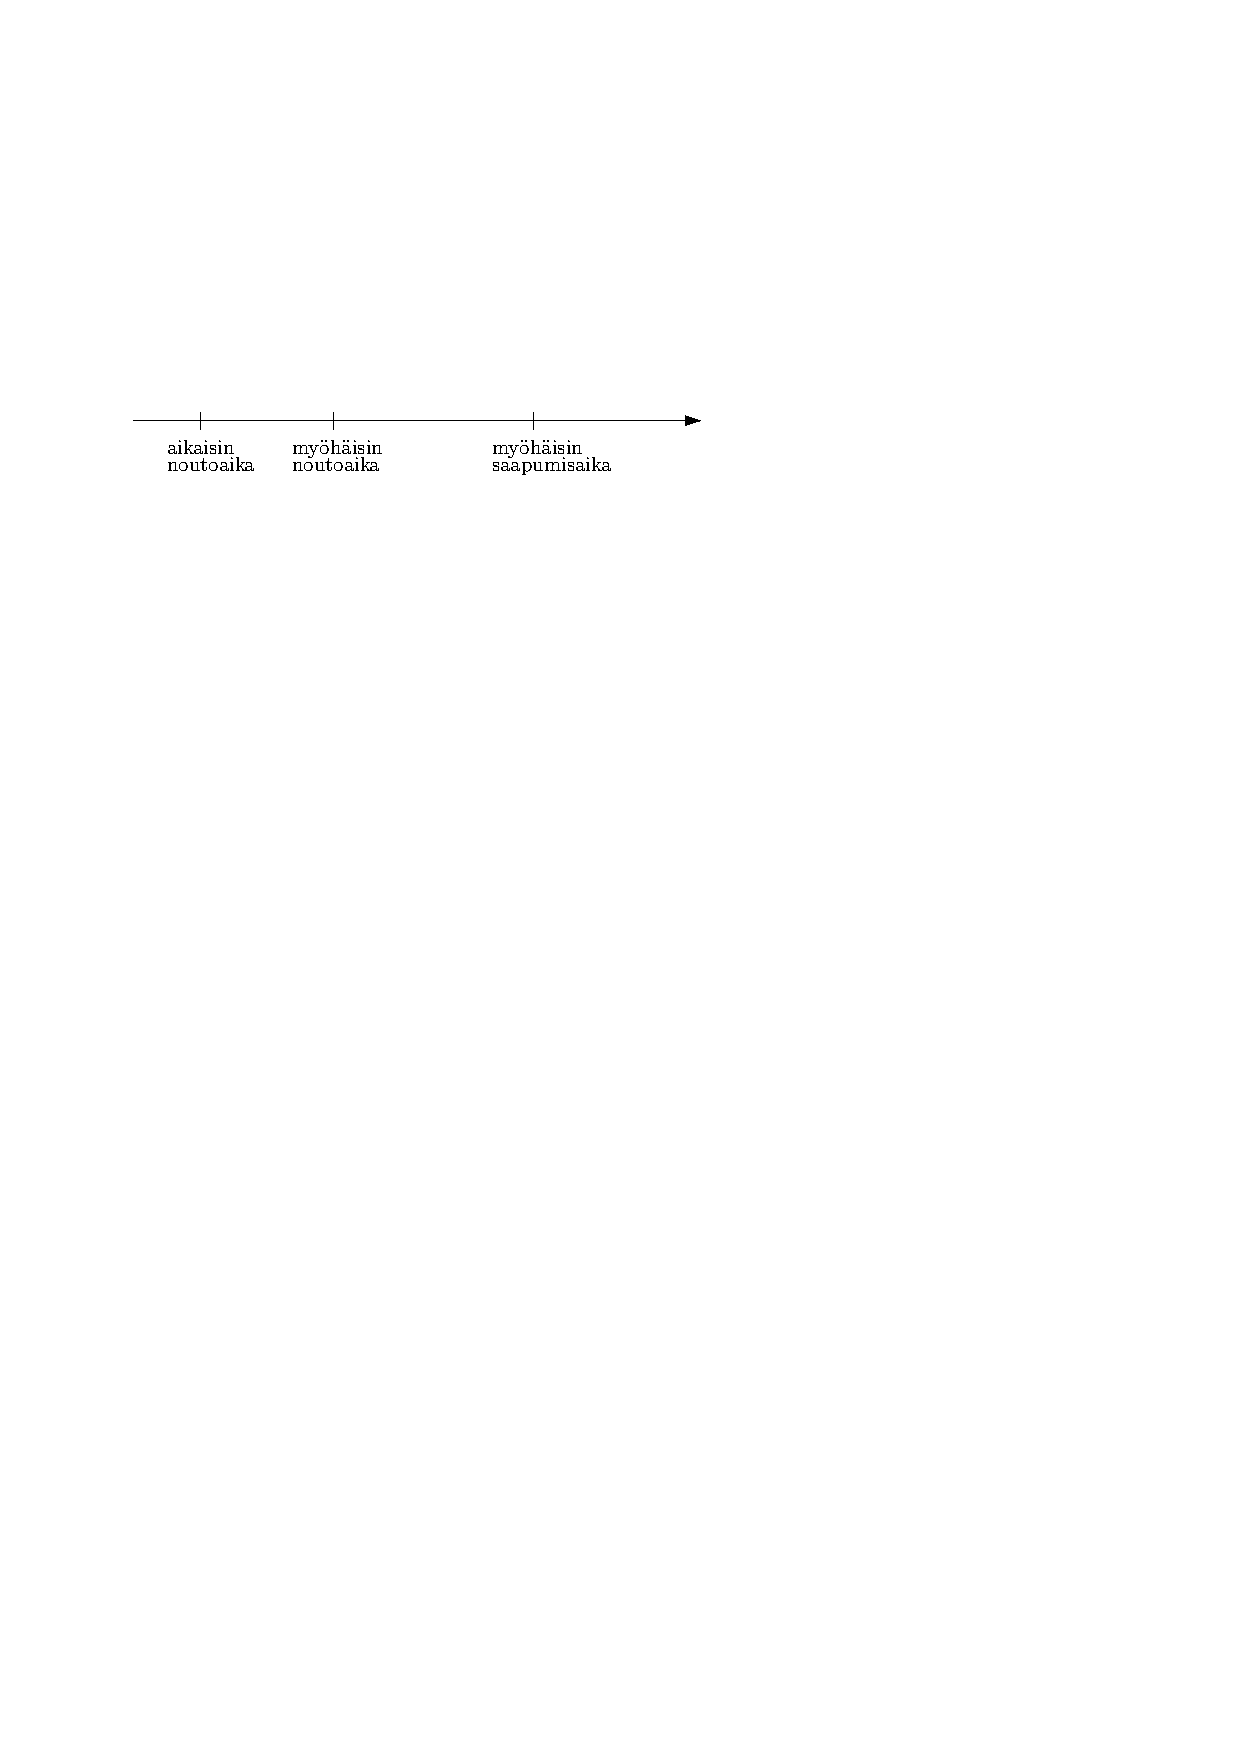
\includegraphics[scale=0.8]{aikaikkuna01}
% \end{center}
% \end{frame}    
%     
    
    
% \begin{frame}
%   \frametitle{Ajoneuvon ja reitin valintaongelma}   % Insert frame title between curly braces
% \begin{itemize}
% 
% %\end{itemize}
% %\begin{center}
% % 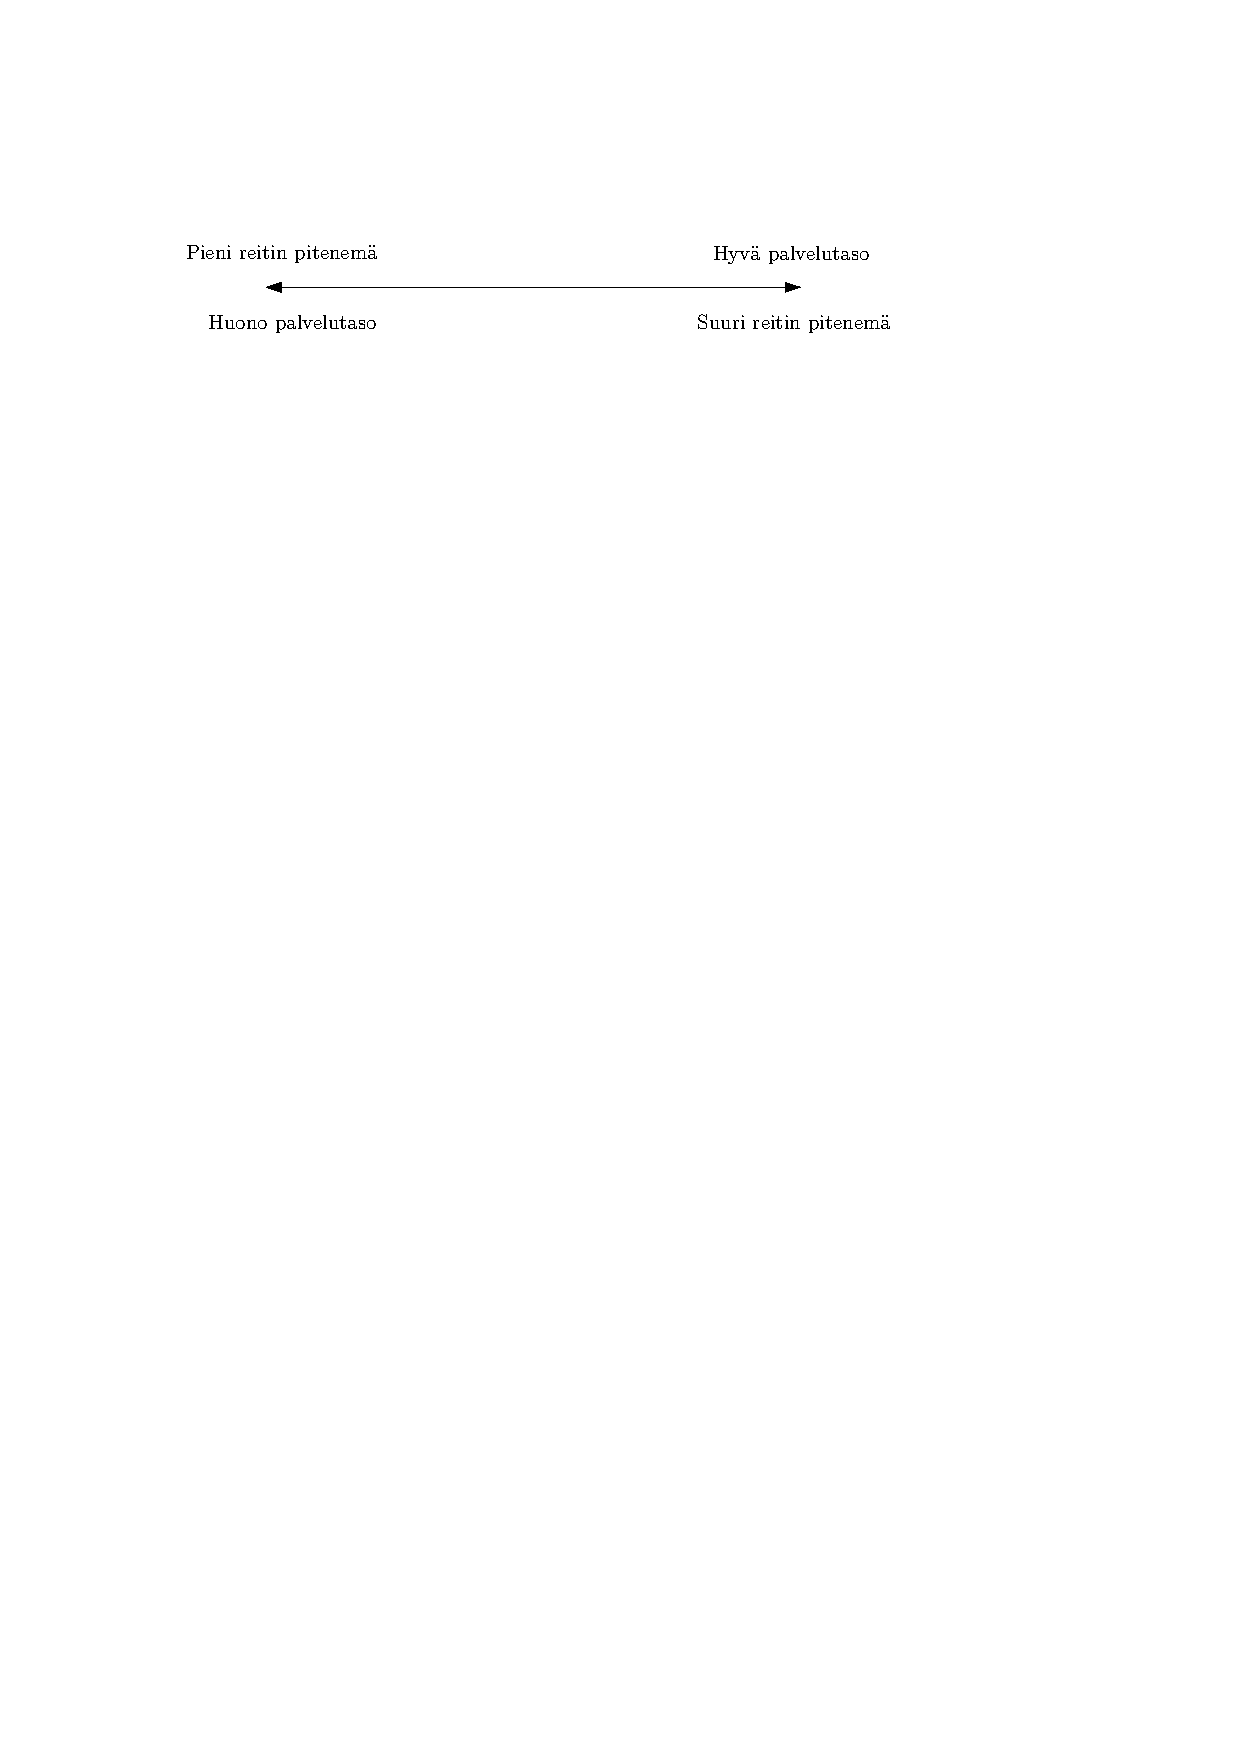
\includegraphics[scale=0.6]{vskuvatavoite}
% %\end{center}
% \item
% Yleisesti jos minimoidaan reitin pituutta, palvelutaso saattaa kärsiä ja jos optimoidaan ainoastaan palvelutasoa, kustannukset kasvavat
% %\begin{itemize}
% \end{itemize}
% \end{frame}

\subsection{Hajautettu ratkaisu}
\begin{frame}
  \frametitle{Hajautettu ratkaisu}   % Insert frame title between curly braces
\begin{itemize}
\item
Yritetään lisätä uusi asiakas johonkin olemassaolevista reiteistä %$\to$ käsitellään jokainen ajoneuvo erikseen
%\item
%Valitaan se ajoneuvo, jonka reitille uusi asiakas sopii parhaiten
\item
Lasketaan jokaiselle ajoneuvolle uusi reittiehdotus ja valitaan niistä paras
\item
Ajoneuvojen reittiehdotukset lasketaan erikseen, toisistaan riippumatta 
\begin{itemize}
 \item 
 Rinnakkaislaskenta
\end{itemize}
%\item
%Asiakkaalle voidaan ilmoittaa ajoneuvon tunniste tilauksen yhteydessä
\end{itemize}
\end{frame}



%                 \begin{frame}
%   \frametitle{Hajautettu ratkaisu, esimerkki}   % Insert frame title between curly braces
% \begin{minipage}[t][0.3\textheight][t]{\textwidth}
%   \begin{itemize}
%  \item 
%  Kaksi ajoneuvoa, joista toinen odottaa tyhjänä
% \end{itemize}
%   \end{minipage}
%   \vfill
%   \begin{minipage}{\textwidth}
%     \centering
% 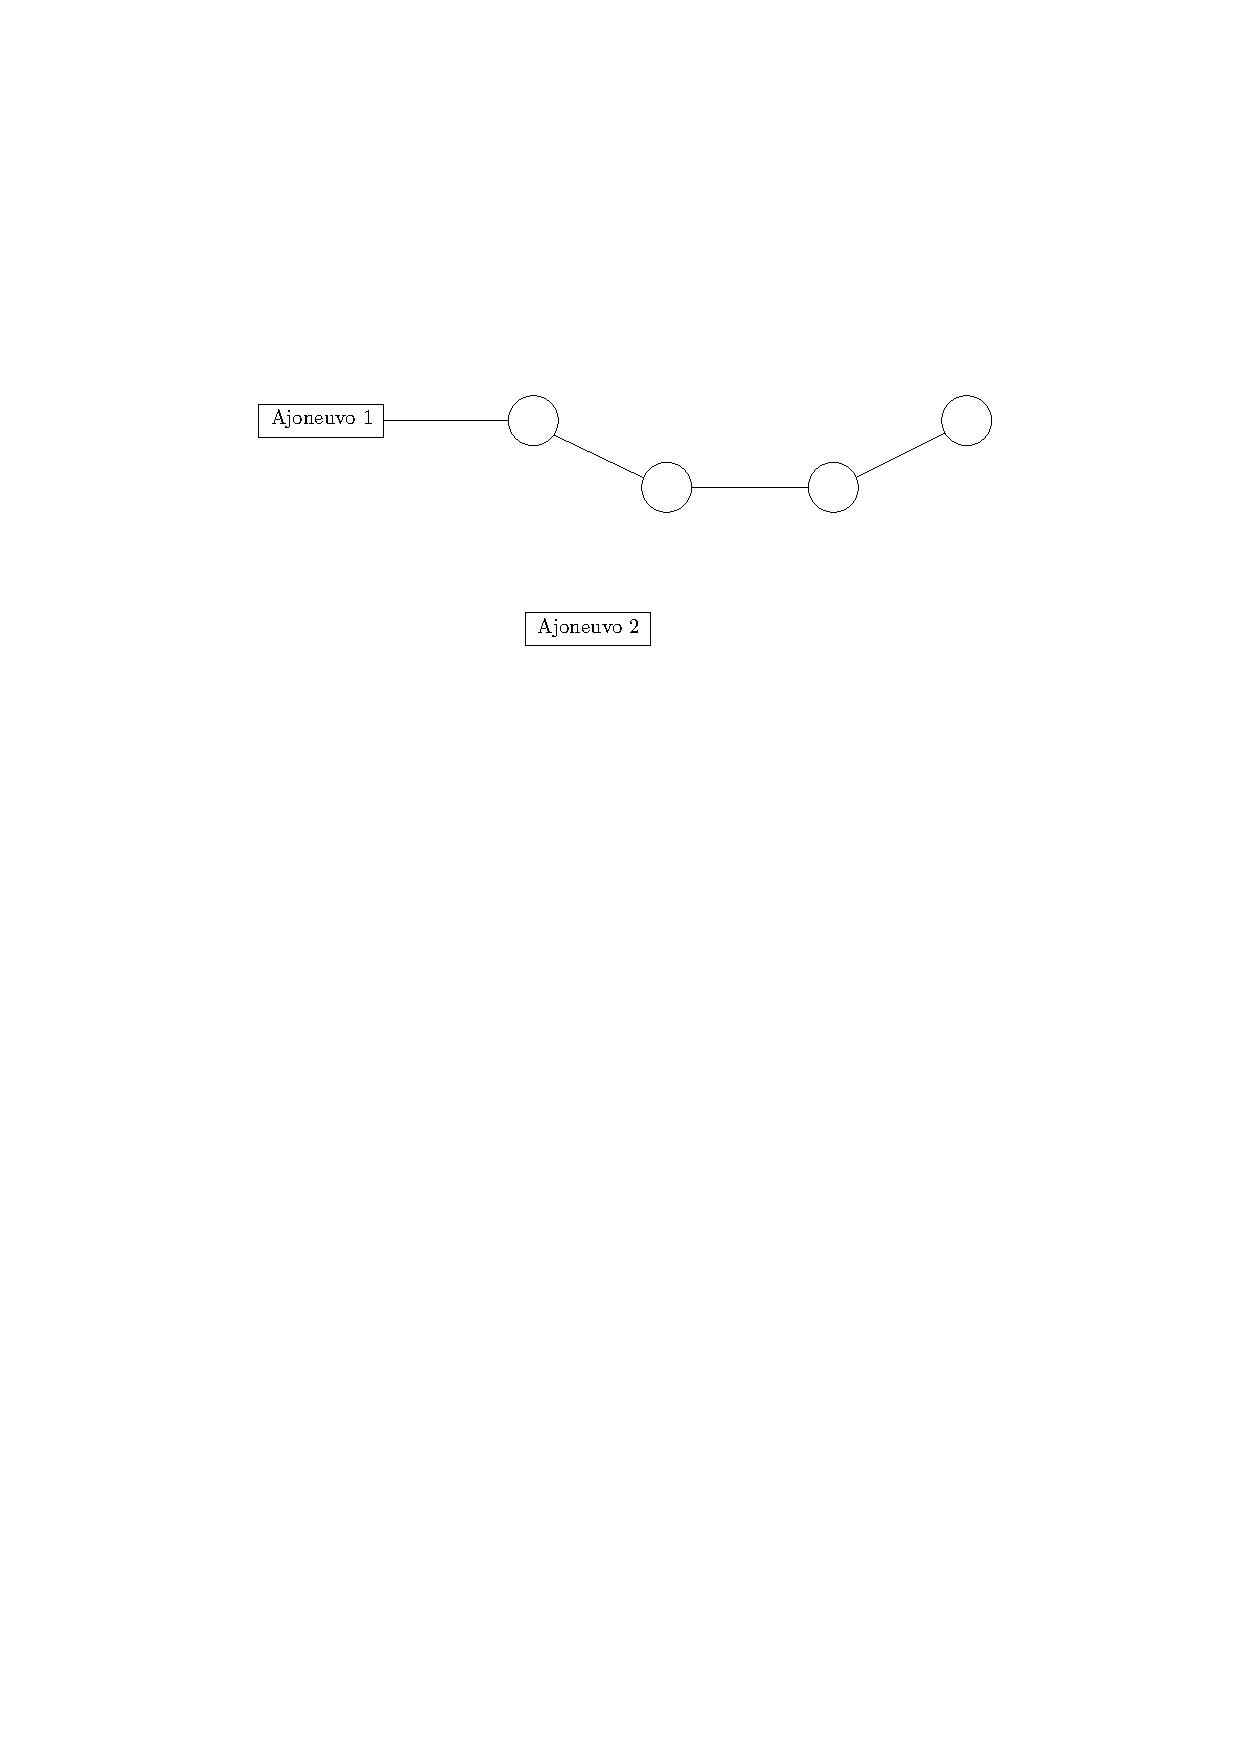
\includegraphics[scale=0.6]{valinta01}
%   \end{minipage}
%     \end{frame}
%     
%     
%                     \begin{frame}
%   \frametitle{Hajautettu ratkaisu, esimerkki}   % Insert frame title between curly braces
% \begin{minipage}[t][0.3\textheight][t]{\textwidth}
%   \begin{itemize}
%  \item 
%  Kaksi ajoneuvoa, joista toinen odottaa tyhjänä
%    \item 
%  Uusi asiakas tilaa matkan ($u^+,u^-$)
% \end{itemize}
%   \end{minipage}
%   \vfill
%   \begin{minipage}{\textwidth}
%     \centering
% 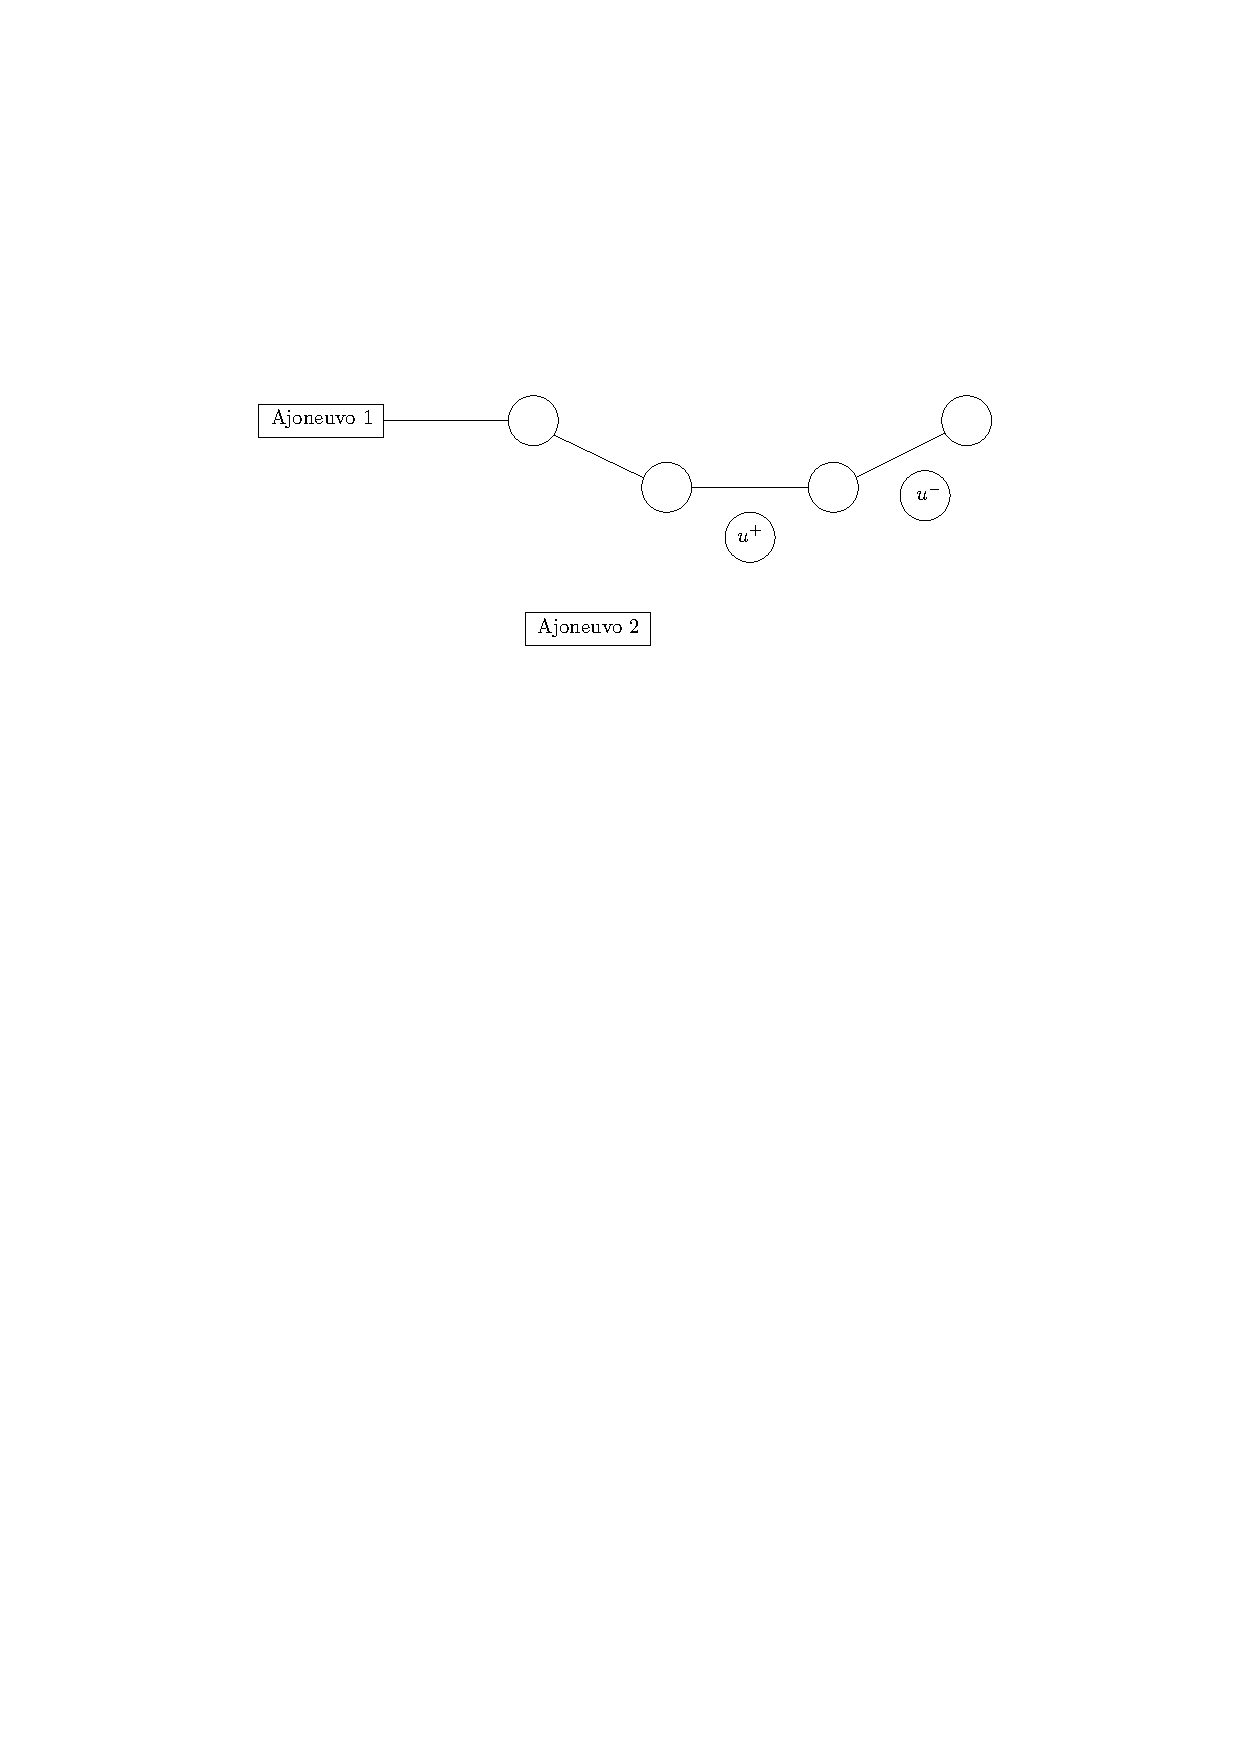
\includegraphics[scale=0.6]{valinta02}
%   \end{minipage}
%   
%   \end{frame}
%     
%                         \begin{frame}
%   \frametitle{Hajautettu ratkaisu, esimerkki}   % Insert frame title between curly braces
% \begin{minipage}[t][0.3\textheight][t]{\textwidth}
%   \begin{itemize}
%  \item 
%  Kaksi ajoneuvoa, joista toinen odottaa tyhjänä
%    \item 
%  Uusi asiakas tilaa matkan ($u^+,u^-$)
%  \item
%  Ehdotus 1: reitin pitenemä minimoituu, palvelutaso kärsii
% \end{itemize}
%   \end{minipage}
%   \vfill
%   \begin{minipage}{\textwidth}
%     \centering
% 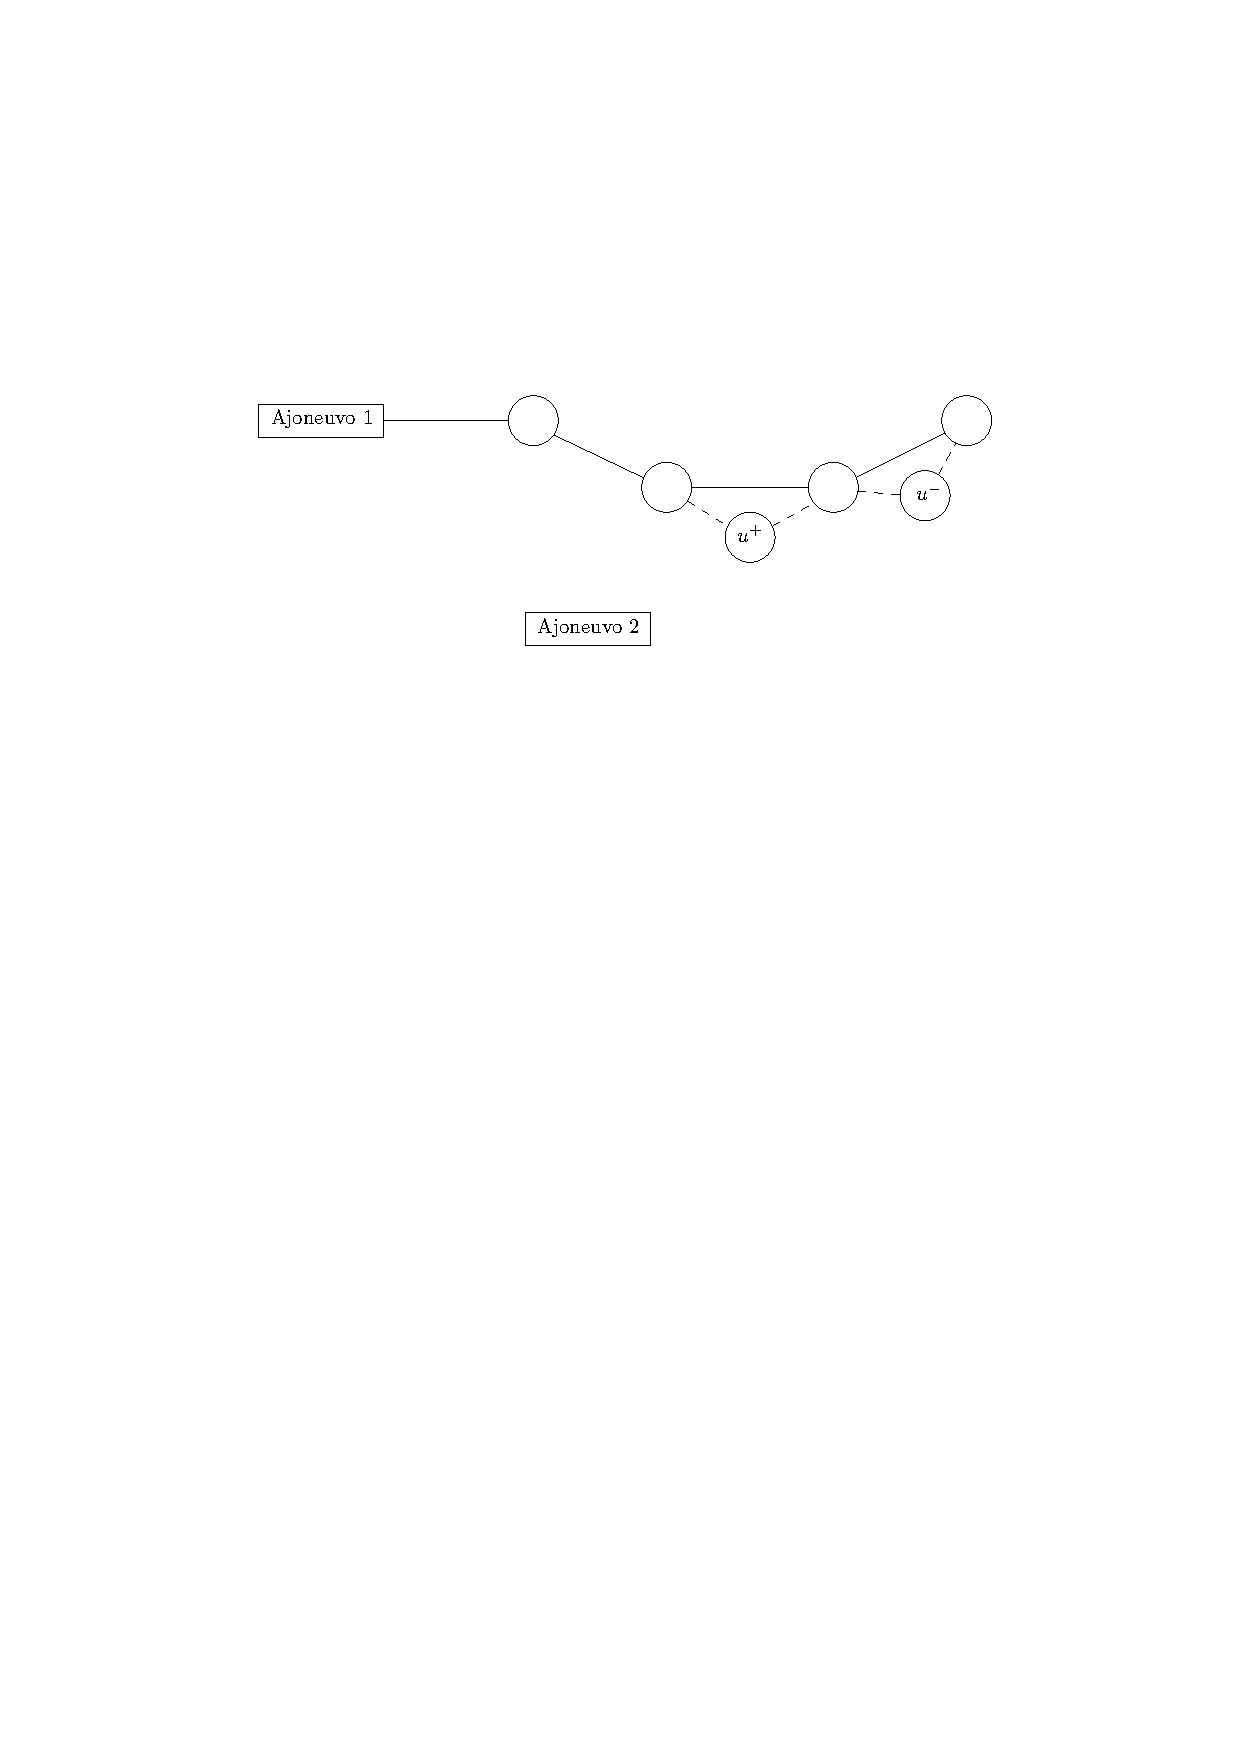
\includegraphics[scale=0.6]{valinta03}
%   \end{minipage}
%   
%   \end{frame}
%   
  \begin{frame}
  \frametitle{Hajautettu ratkaisu, esimerkki}   % Insert frame title between curly braces
  \begin{itemize}
%  \item 
%  Kaksi ajoneuvoa, joista toinen odottaa tyhjänä
%    \item 
%  Uusi asiakas tilaa matkan ($u^+,u^-$)
 \item
 Ehdotus 1: reitin pitenemä minimoituu, palvelutaso kärsii
 \end{itemize}
 
    \begin{minipage}{\textwidth}
    \centering
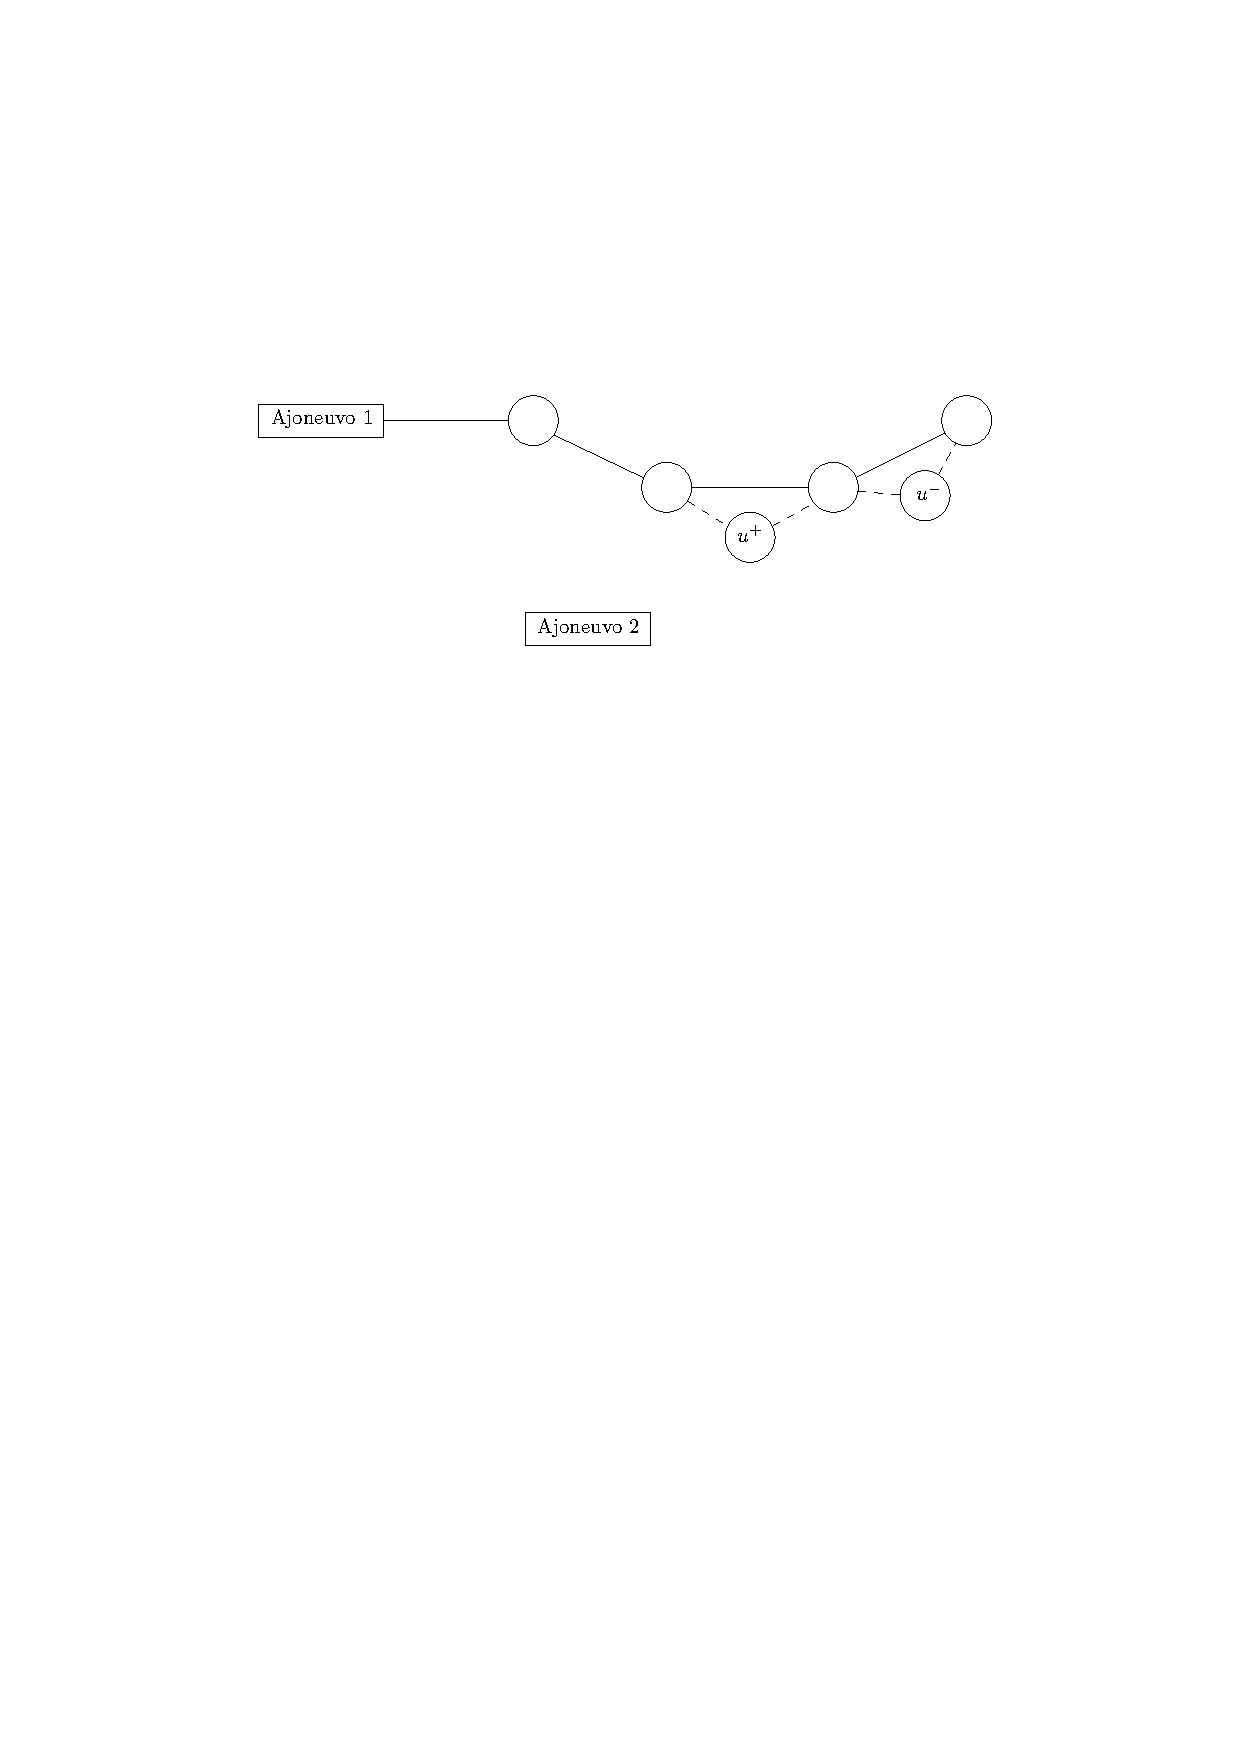
\includegraphics[scale=0.5]{valinta03}
  \end{minipage}
\begin{itemize}
  \item
 Ehdotus 2: palvelutaso on paras mahdollinen, reitin pituus kasvaa enemmän
\end{itemize}

  \vfill
  \begin{minipage}{\textwidth}
    \centering
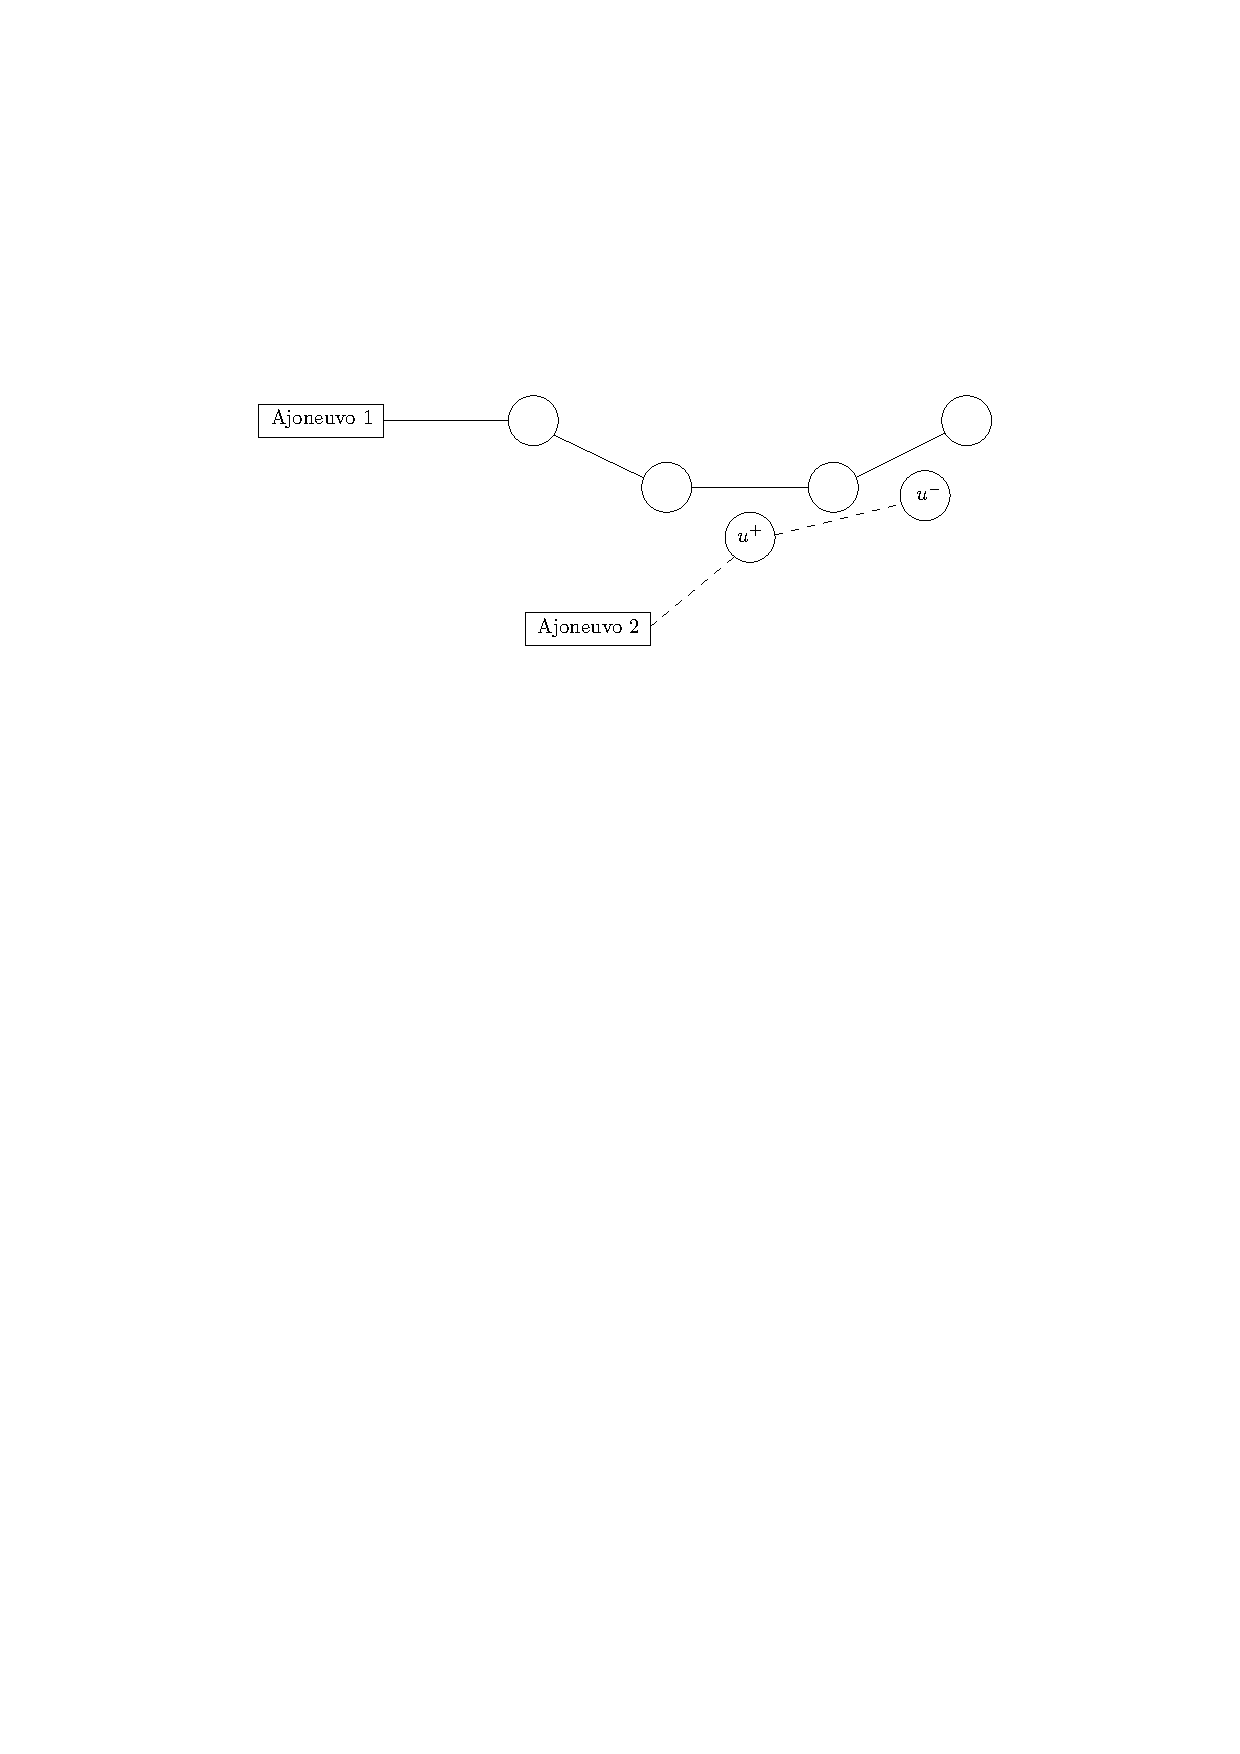
\includegraphics[scale=0.5]{valinta04}
  \end{minipage}
  
  \end{frame}
    

%     \begin{frame}
% \frametitle{Yksinkertainen lisäysalgoritmi (Insertion algorithm)}
%  \begin{itemize}
% \item
% Yksinkertainen ratkaisu reittiehdotusten laskemiselle on lisätä uuden asiakkaan nouto- ja toimituspiste sopivaan väliin 
% \item
% Ei-täydellinen ratkaisu: olemassaolevien pisteiden järjestys säilyy
% \end{itemize}
% \begin{center}
%  \includegraphics[scale=0.5]<1>{insertion02}
%   \includegraphics[scale=0.5]<2>{insertion03}
%    \includegraphics[scale=0.5]<3>{insertion04}
%     \includegraphics[scale=0.5]<4>{insertion05}
%       \includegraphics[scale=0.5]<5>{insertion06}
%        \includegraphics[scale=0.5]<6>{insertion07}
%         \includegraphics[scale=0.5]<7>{insertion08}
%          \includegraphics[scale=0.5]<8>{insertion09}
% 
%            
% \end{center}
% 
% \end{frame}
%     
%     \begin{frame}
% \frametitle{Laajennettu lisäysalgoritmi (Adaptive insertion algorithm)}
%  \begin{itemize}
% \item
% Rakennetaan lisäysperiaatteella rinnakkain useampi vaihoehtoinen reitti ja valitaan niistä paras
% \end{itemize}
% \begin{center}
%  \includegraphics[scale=0.5]<1>{insertion02}
%   \includegraphics[scale=0.5]<2>{insertion03}
%    \includegraphics[scale=0.5]<3>{insertion04}
%     \includegraphics[scale=0.5]<4>{insertion05}
%      \includegraphics[scale=0.5]<5>{insertion06}
%       \includegraphics[scale=0.5]<6>{insertion07}
%        \includegraphics[scale=0.5]<7>{insertion08}
%        \includegraphics[scale=0.5]<8>{insertion09}
% \\
% \hfill
% \\
% \hfill
% \\
%                 \includegraphics[scale=0.5]<1>{insertion02}   
%                 \includegraphics[scale=0.5]<2>{insertion03}
%                 \includegraphics[scale=0.5]<3>{insertion04}  
%                 \includegraphics[scale=0.5]<4>{insertion05}
%                 \includegraphics[scale=0.5]<5>{insertion06b} 
%                 \includegraphics[scale=0.5]<6>{insertion07b} 
%                 \includegraphics[scale=0.5]<7>{insertion08b} 
%                 \includegraphics[scale=0.5]<8>{insertion09b} 
% \end{center}
% 
% \end{frame}
% 
% 
%     \begin{frame}
% \frametitle{Täydellinen lisäysalgoritmi (Exact insertion algorithm)}
%  \begin{itemize}
%  \item
% Rakennetaan lisäysperiaatteella rinnakkain kaikki mahdolliset reitit (enintään $\frac{(2n)!}{2^n}$ kpl)
% \item
% Osa reiteistä voidaan hylätä rajoitusten perusteella
% %\item
% %Perusidea: luetellaan yhden ajoneuvon kaikki mahdolliset reitit ja valitaan niistä paras 
% %\item
% %Kaikki mahdolliset reitit ($\frac{(2n)!}{2^n}$ kpl) saadaan lisäämällä asiakkaat yksi kerrallaan \emph{kaikkiin edellisiin} reitteihin
% \end{itemize}
% \hfill \\
%   \begin{columns}[c]
%   \column{0.7in}
%   \column{2.5in}  % slides are 3in high by 5in wide
%  $1^+,1^-$ \\
%  \hfill \\
%   $1^+,1^-,2^+,2^-$ \\
%     $1^+,2^+,1^-,2^-$ \\
%      $1^+,2^+,2^-,1^-$ \\
%       $2^+,1^+,1^-,2^-$ \\
%       $2^+,1^+,2^-,1^-$ \\
%       $2^+,2^-,1^+,1^-$ \\
%       \column{2.5in}
%       {\tiny 
%         $1^+,1^-,2^+,2^-,3^+,3^-$ \\
%         $1^+,1^-,2^+,3^+,2^-,3^-$ \\
%         $1^+,1^-,3^+,2^+,2^-,3^-$ \\
%         $1^+,3^+,1^-,2^+,2^-,3^-$ \\
%         $3^+,1^+,1^-,2^+,2^-,3^-$ \\
%         
%         $1^+,1^-,2^+,3^+,3^-,2^-$ \\
%         $1^+,1^-,3^+,2^+,3^-,2^-$ \\
%         $1^+,3^+,1^-,2^+,3^-,2^-$ \\
%         $3^+,1^+,1^-,2^+,3^-,2^-$ \\
%         
%         $1^+,1^-,3^+,3^-,2^+,2^-$ \\
%         $1^+,3^+,1^-,3^-,2^+,2^-$ \\
%         $3^+,1^+,1^-,3^-,2^+,2^-$ \\
%         
%       \ldots
%       }
%       \end{columns}
% \end{frame}
%     
    
    
%     \begin{frame}
% \frametitle{Täydellinen lisäysalgoritmi (Exact insertion algorithm)}
%  \begin{itemize}
%  \item
% Rakennetaan lisäysperiaatteella rinnakkain kaikki mahdolliset reitit (enintään $\frac{(2n)!}{2^n}$ kpl)
% \item
% Osa reiteistä voidaan hylätä rajoitusten perusteella
% %\item
% %Perusidea: luetellaan yhden ajoneuvon kaikki mahdolliset reitit ja valitaan niistä paras 
% %\item
% %Kaikki mahdolliset reitit ($\frac{(2n)!}{2^n}$ kpl) saadaan lisäämällä asiakkaat yksi kerrallaan \emph{kaikkiin edellisiin} reitteihin
% \end{itemize}
% \hfill \\
%   \begin{columns}[c]
%   \column{0.7in}
%   \column{2.5in}  % slides are 3in high by 5in wide
%  $1^+,1^-$ \\
%  \hfill \\
%   $1^+,1^-,2^+,2^-$ \\
%     $\cancel{1^+,2^+,1^-,2^-}$ \\
%      $1^+,2^+,2^-,1^-$ \\
%       $\cancel{2^+,1^+,1^-,2^-}$ \\
%       $\cancel{2^+,1^+,2^-,1^-}$ \\
%       $2^+,2^-,1^+,1^-$ \\
%       \column{2.5in}
%       {\tiny 
%         $1^+,1^-,2^+,2^-,3^+,3^-$ \\
%         $1^+,1^-,2^+,3^+,2^-,3^-$ \\
%         $\cancel{1^+,1^-,3^+,2^+,2^-,3^-}$ \\
%         $\cancel{1^+,3^+,1^-,2^+,2^-,3^-}$ \\
%         $3^+,1^+,1^-,2^+,2^-,3^-$ \\
%         
%         $1^+,1^-,2^+,3^+,3^-,2^-$ \\
%         $1^+,1^-,3^+,2^+,3^-,2^-$ \\
%         $\cancel{1^+,3^+,1^-,2^+,3^-,2^-}$ \\
%         $3^+,1^+,1^-,2^+,3^-,2^-$ \\
%         
%         $\cancel{1^+,1^-,3^+,3^-,2^+,2^-}$ \\
%         $1^+,3^+,1^-,3^-,2^+,2^-$ \\
%         $3^+,1^+,1^-,3^-,2^+,2^-$ \\
%         \
%       \ldots
%       }
%       \end{columns}
% \end{frame}    
%     
%     
%     
%     
%     
%     
%     
    
    
%         \begin{frame}
% \frametitle{Lisäysalgoritmi, tuloksia}
%  \begin{itemize}
% \item
% Tiukkojen aika- tai kapasiteettirajoitusten vallitessa kaikkien mahdollisten reittien lukumäärä pysyy kohtuullisena ja 
% täydellinen algoritmi tuottaa nopeasti optimaalisen ratkaisun
% \item
% Jos rajoitukset eivät ole tiukkoja, saadaan tehokas ratkaisu
% rajoittamalla rinnakkaisten reittien lukumäärää
% \end{itemize}
% \hfill \\
% \begin{center}
% 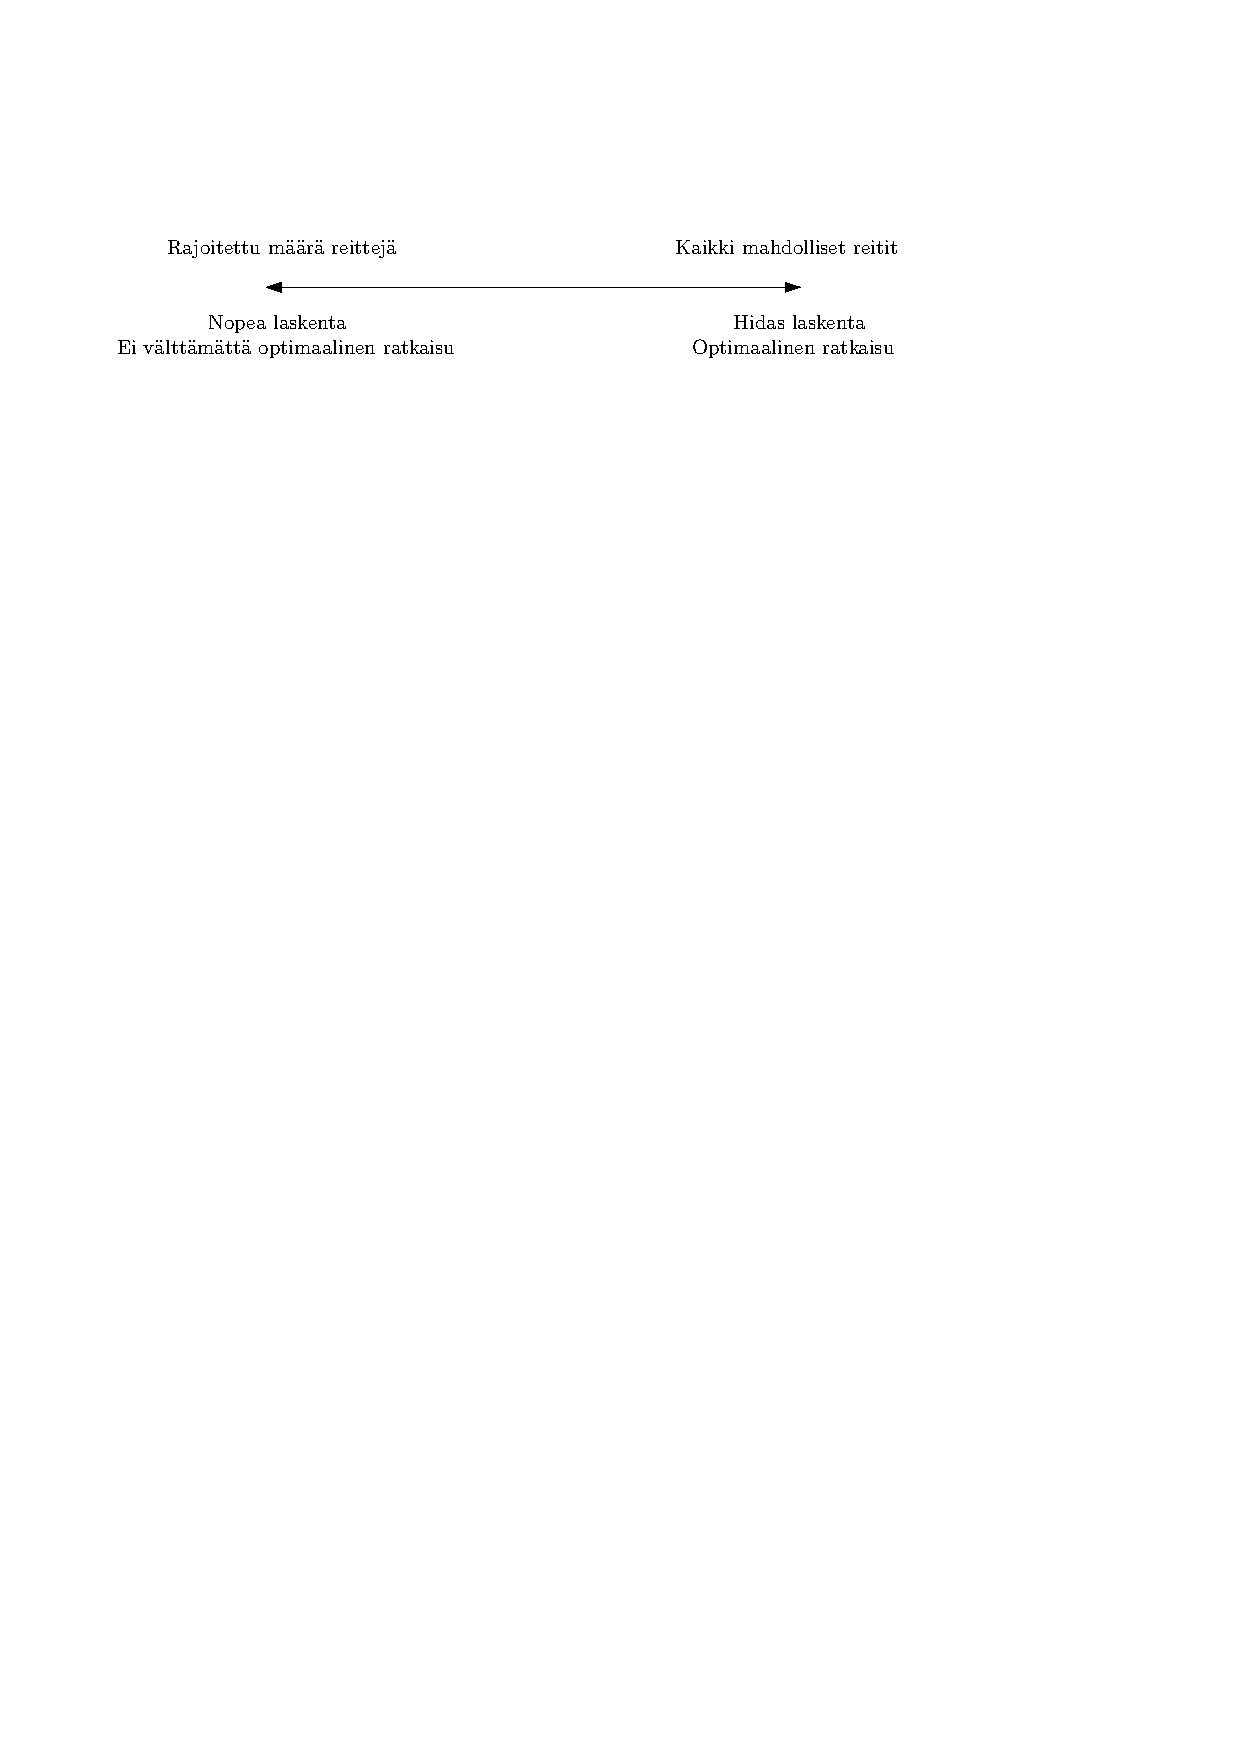
\includegraphics[scale=0.7]{vskuva}
% \end{center}
% \begin{itemize}
%  \item 
%  Yksinkertainen lisäysalgoritmi on täydellinen, kun $n < 3$
% \end{itemize}
% 
% \end{frame}
    
\subsection{Keskitetty ratkaisu}
\begin{frame}
  \frametitle{Keskitetty ratkaisu}   % Insert frame title between curly braces
\begin{itemize}
\item
Uuden matkatilauksen saapuessa etsitään parasta mahdollista asiakkaiden, ajoneuvojen ja reittien yhdistelmää
\item
Toistaiseksi noutamattomien asiakkaiden ajoneuvo voi vaihtua
\end{itemize}
  \begin{minipage}{\textwidth}
    \centering
    \fbox{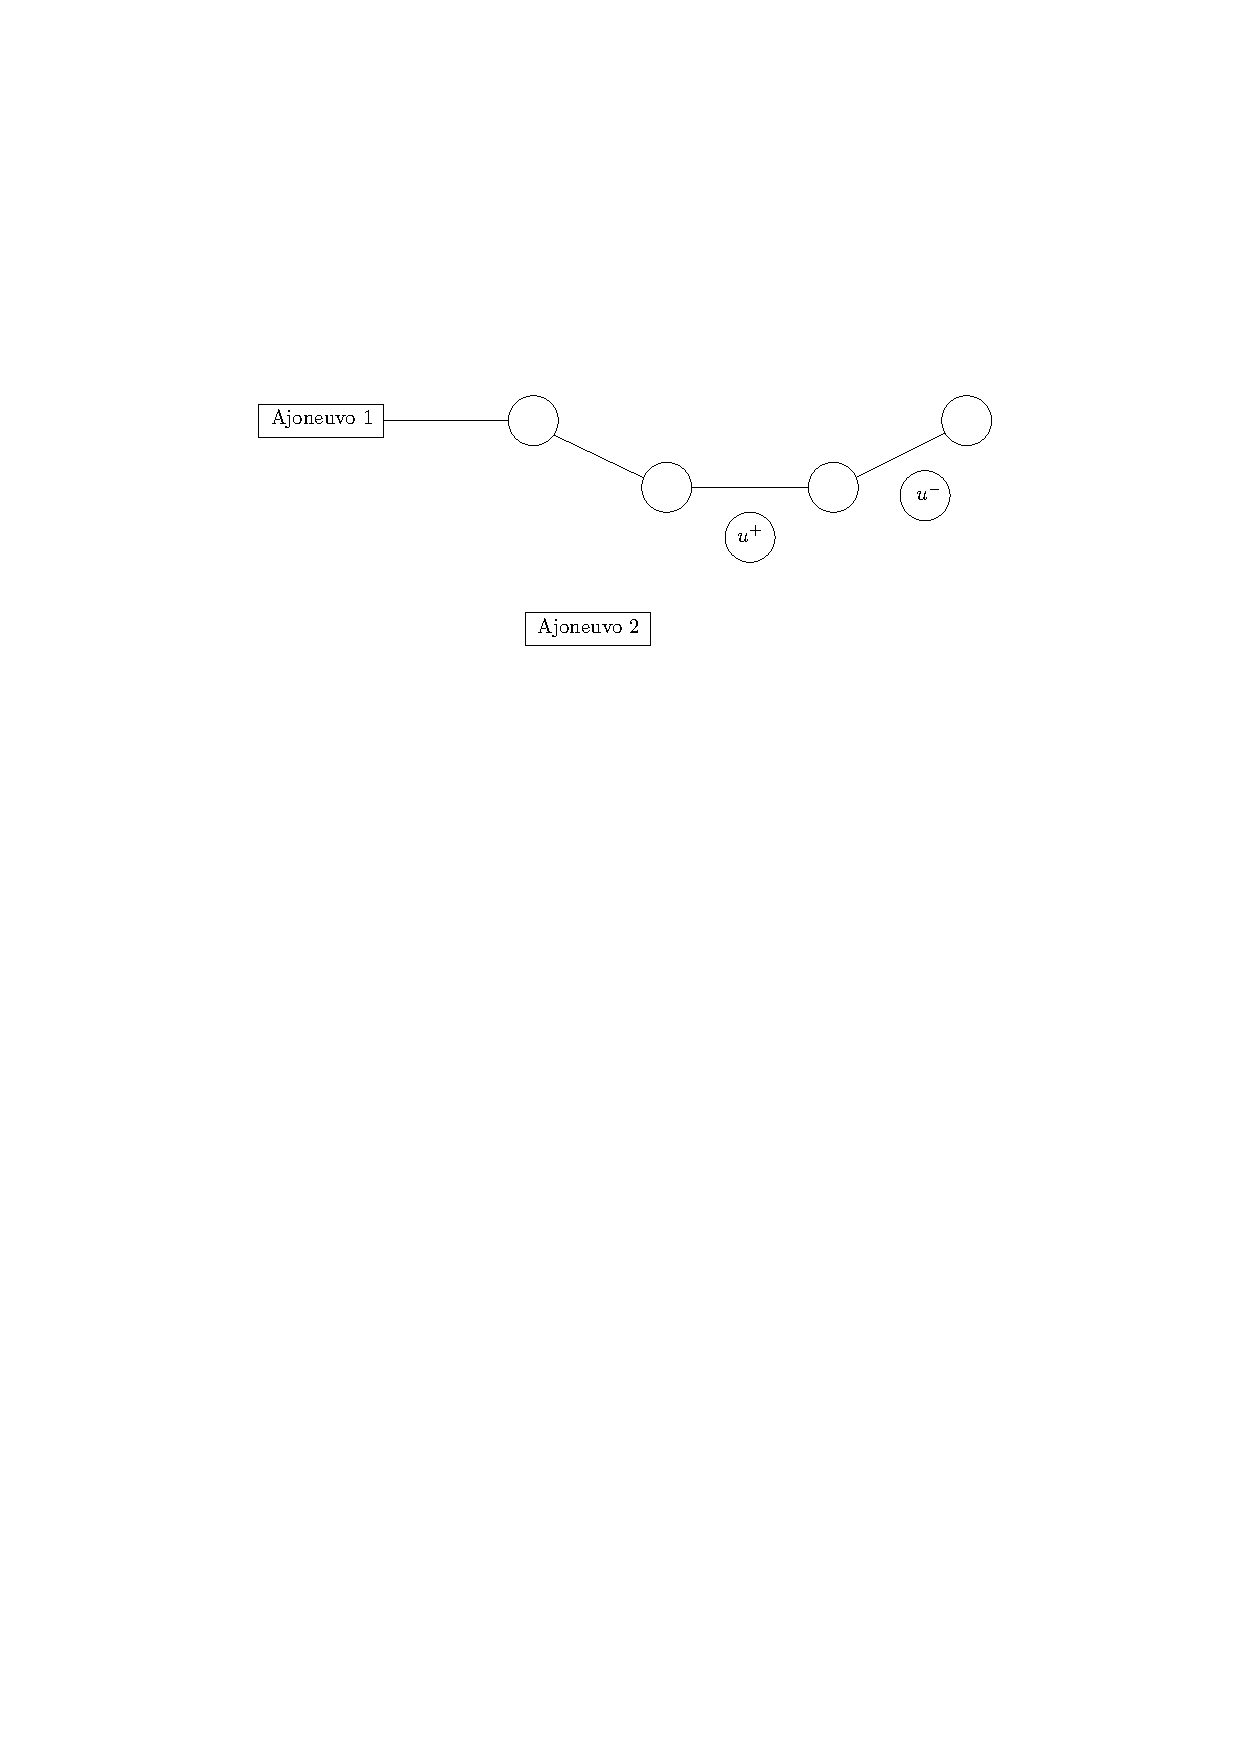
\includegraphics[scale=0.4]{valinta02}} \\
    \hfill \\
\fbox{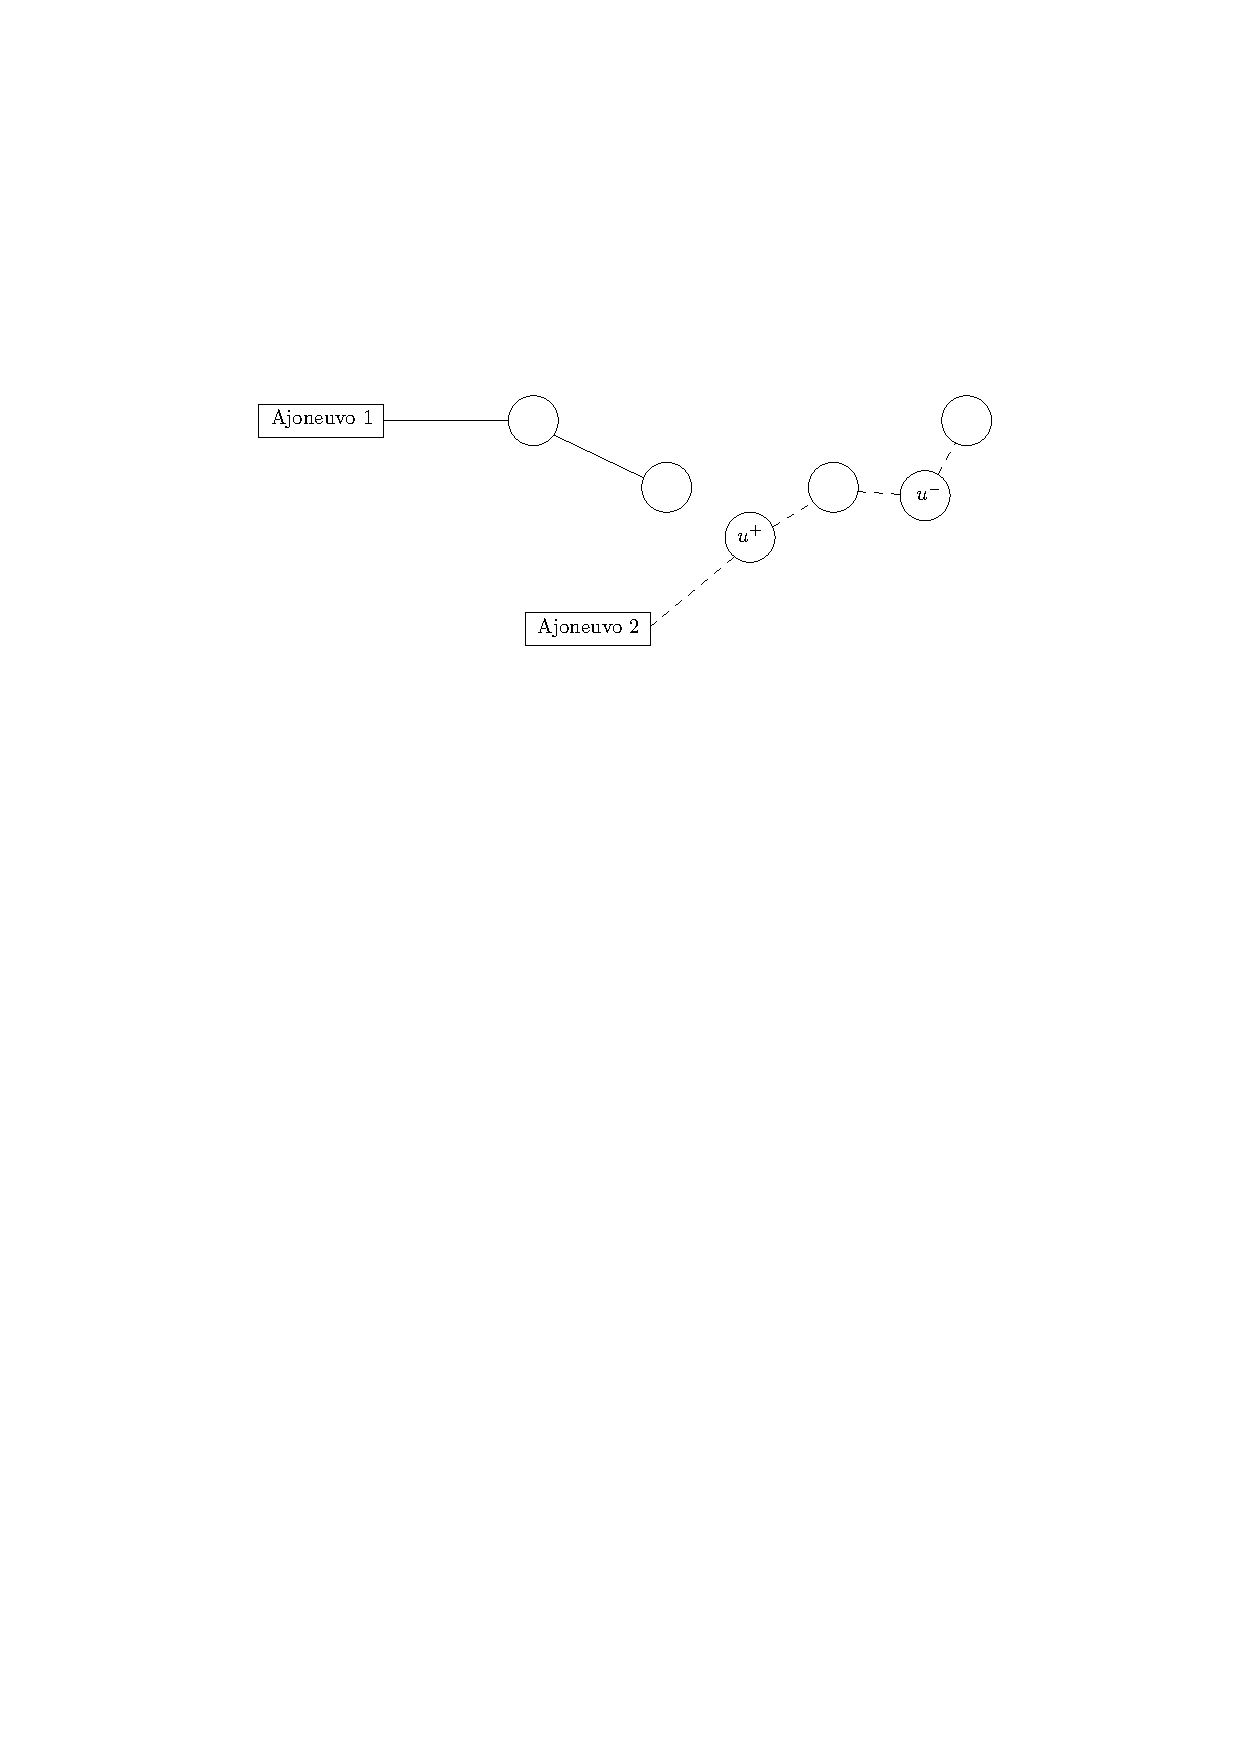
\includegraphics[scale=0.4]{valinta05}}
  \end{minipage}
\end{frame}    
    
% \begin{frame}
%   \frametitle{Keskitetty ratkaisu, esimerkki 2} 
%   \begin{itemize}
%    \item 
%    Keskitetyn ratkaisun merkitys korostuu rajoitetuissa tapauksissa 
%   \end{itemize}
%     \begin{center}
%     \includegraphics[scale=0.7]<1>{keskitettyesim01}
%     \includegraphics[scale=0.7]<2>{keskitettyesim02} 
%     \includegraphics[scale=0.7]<3>{keskitettyesim03} 
%     \includegraphics[scale=0.7]<4>{keskitettyesim04} 
%     \end{center}
% \end{frame}    

\begin{frame}
  \frametitle{Maksimiklusteriperiaate (Maximum cluster algorithm)} 
  \begin{itemize}
   \item 
   Etsitään suurin asiakasjoukko (klusteri), joka sopii yhden ajoneuvon reitille 
   \item
   Uuden matkatilauksen saapuessa klusterit lasketaan uudelleen
  \end{itemize}
  \begin{center}
%       \includegraphics[scale=0.5]<1>{maxcesim04}
%       \includegraphics[scale=0.5]<2>{maxcesim03}
%       \includegraphics[scale=0.5]<3>{maxcesim02}
      \includegraphics[scale=0.5]<1>{maxcesim01}
      \end{center}
\end{frame}  


\begin{frame}
  \frametitle{Arvojärjestysmenetelmä (Routing by Ranking)} 
  \begin{itemize}
   \item 
   Maksimiklusterit voidaan määrittää tehokkaasti järjestämällä nouto- ja toimituspisteet arvojärjestykseen
   \item
   Suurimman arvon saavat pisteet, joista on mahdollista siirtyä mahdollisimman moneen arvokkaaseen pisteeseen aikarajojen sisällä
   \item
   Arvojärjestys saadaan laskemalla suurinta ominaisarvoa vastaava ominaisvektori (ks. HITS-hakualgoritmi)
  \end{itemize}
  \begin{center}
       \includegraphics[scale=0.5]<1>{hub01}
%       \includegraphics[scale=0.5]<2>{hub02}
      \includegraphics[scale=0.5]<2>{hub03}
      \end{center}
\end{frame}  

\begin{frame}
  \frametitle{Keskitetty ratkaisu, tuloksia} 
  \begin{itemize}
   \item 
    Arvojärjestysmenetelmä tuottaa tehokkaasti käypiä ratkaisuja tiukkojen rajoitusten vallitessa 
    \item
    Kertaluokkaa nopeampi aikaisempiin menetelmiin verrattuna
    \item
    Yleisesti keskitetyn ratkaisun merkitys korostuu, kun
    \begin{itemize}
     \item 
     rajoitteet ovat tiukkoja
     \item
     reitit ovat pitkiä (pitkät ennakkotilausajat)
    \end{itemize}
   \end{itemize}
\end{frame}  

% \begin{frame}
%   \frametitle{Hajautetun ja keskitetyn ratkaisun vertailu} 
%   \begin{itemize}
%    \item 
% Hajautettu ratkaisu 
% \begin{itemize}
% \item
% Laskennallisesti kevyempi
% \item
% Palvelutason kannalta luotettavampi
% \end{itemize}
% 
% \item
% Keskitetty ratkaisu
%    \begin{itemize}
% \item
% Parempi kustannustehokkuus
% \item
% Ajoneuvon vaihto ennen noutoa lisää palvelutason epävarmuutta
% \end{itemize}
%    \end{itemize}
% \end{frame}  





\section{Matkansuunnittelu}
\frame{\secpage}
\subsection{Matkansuunnittelun mallit}
\begin{frame}
  \frametitle{Matkansuunnittelu} 
  \begin{itemize}
   \item 
    Matkansuunnittelu (Journey planning) = joukkoliikennevälineen ja reitin valinta
    \item
    Tarkoituksena on löytää matkustajalle paras reitti ja aikataulu lähtöpisteestä määränpäähän, esim.
    \begin{itemize}
     \item 
     16:27: kävely pysäkille A,
     \item
     16:39: bussi numero 58 pysäkiltä A pysäkille B
     \item
     16:53: kävely pysäkiltä B määränpäähän, perillä klo 17:11
    \end{itemize}
   \end{itemize}
     \begin{center}
      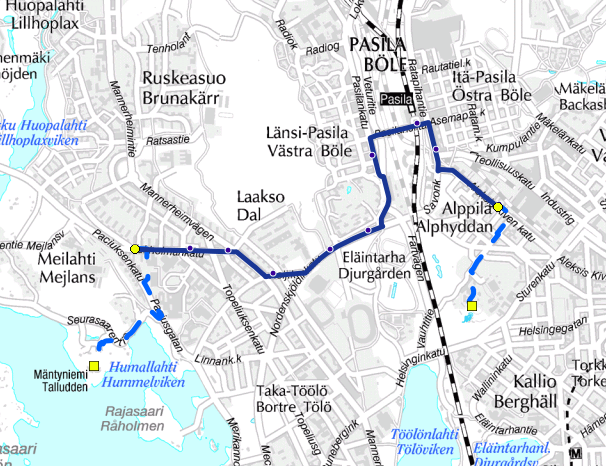
\includegraphics[scale=0.2]{reittiopas01}
      \end{center}
\end{frame} 

\begin{frame}
 \frametitle{Lyhimmän polun ongelma (Shortest Path Problem)} 
 \begin{columns}
 \column{2.5in}
  \begin{itemize}
\item
Matkansuunnitteluongelma muistuttaa niin sanottua lyhimmän polun ongelmaa 
\item
Tarkoituksena on löytää lyhin mahdollinen polku kahden pisteen välillä
\item
Kauppamatkustajan ongelmaan verrattuna lyhimmän polun ongelma on helpompi
\end{itemize}
    \column{2.5in}
\centering

%\framebox{
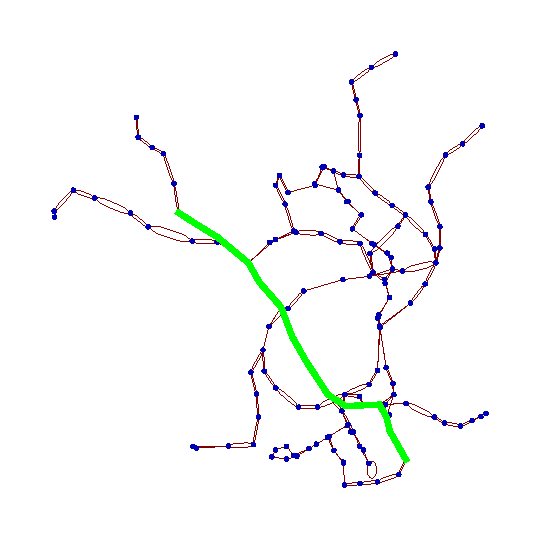
\includegraphics[scale=0.6]{shortestpathexample}
%}
 
  \end{columns}

\end{frame}


\begin{frame}
  \frametitle{Deterministinen ja stokastinen malli} 
  \begin{itemize}
   \item 
    \emph{Deterministisillä} menetelmillä voidaan laskea etukäteen paras reitti esim. matka-ajan, odotusajan, kävelymatkan tai vaihtojen lukumäärän suhteen 
    \item
    Todellisuudessa etukäteen laskettu reitti ei välttämättä toteudu esim. myöhästymisien tai vuorojen peruutuksien takia
    \item
    \emph{Stokastinen} malli ottaa huomioon mahdolliset reittimuutokset matkan varrella
    \item
    Mallin avulla voidaan laskea parhaan reitin lisäksi paras matkastrategia eri tavoitteiden suhteen
   \end{itemize}
     \begin{center}
      \end{center}
\end{frame} 

% \begin{frame}
%   \frametitle{Deterministinen malli, esimerkki} 
%   \begin{minipage}[t][0.3\textheight][t]{\textwidth}
%   \begin{itemize}
%    \item 
% Tavoitteena on saapua mahdollisimman aikaisin määränpäähän, vaihto pysäkillä A tai B
% \item
% Kaikki bussilinjat kulkevat 20 minuutin välein
% \item
% Nopein matka: bussi 1 klo 15:00, vaihto pysäkillä A, perillä klo 15:30
%    \end{itemize}
%    \end{minipage}
%    \vfill
%      \begin{minipage}{\textwidth}
%      \begin{center}
%      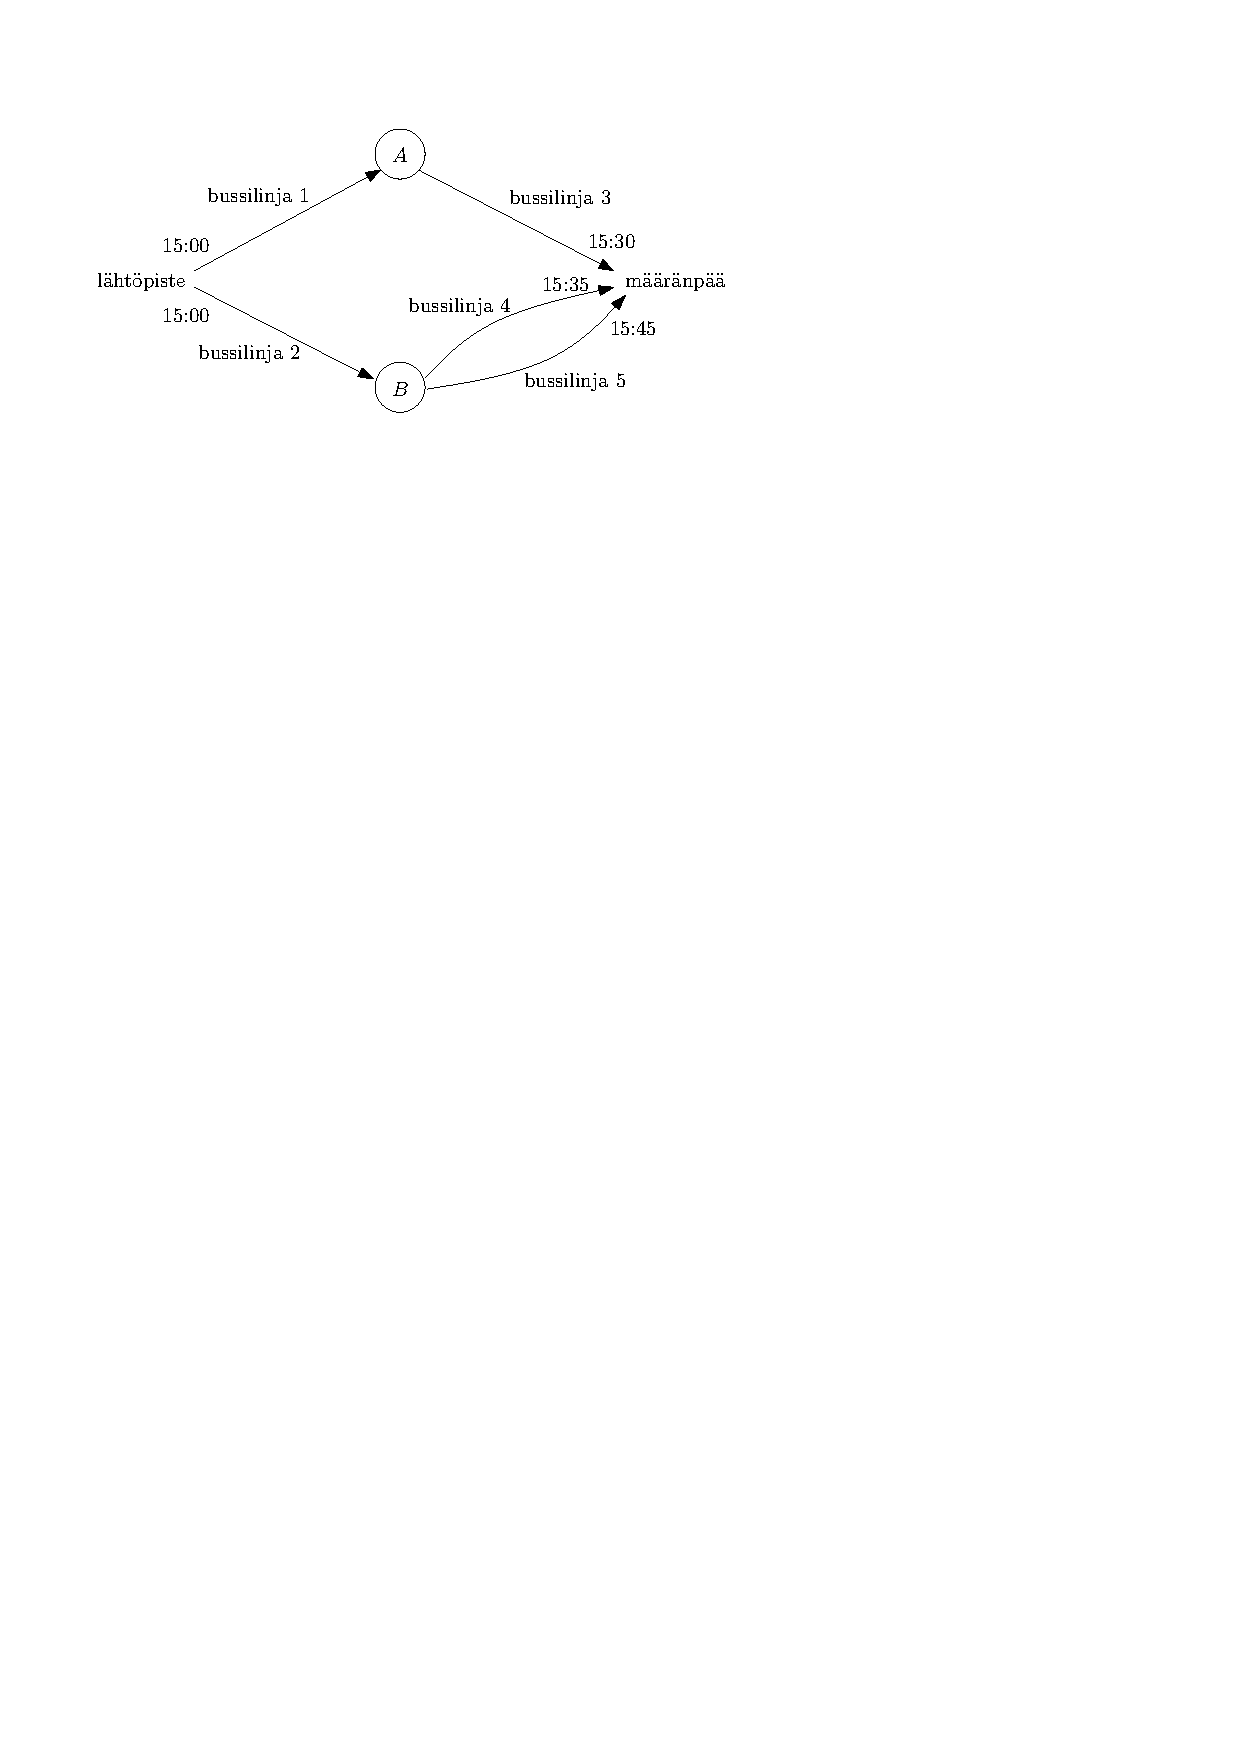
\includegraphics[scale=0.6]{matkansuunnittelu01}
%       \end{center}
%       \end{minipage}
% \end{frame} 
% 
% \begin{frame}
%   \frametitle{Stokastinen malli, esimerkki} 
%   \begin{minipage}[t][0.3\textheight][t]{\textwidth}
%   \begin{itemize}
%    \item 
% Lisätään malliin vaihtojen onnistumisien todennäköisyydet 
% \item
% Jos kuljetaan busseilla 1 ja 3 pysäkin A kautta, saapumisajan odotusarvo on 15:40
% \item
% Paras matkastrategia: bussilla 2 pysäkille B, vaihto seuraavaksi saapuvaan bussiin, odotettu saapumisaika 15:37
%    \end{itemize}
%    \end{minipage}
%    \vfill
%      \begin{minipage}{\textwidth}
%      \begin{center}
%      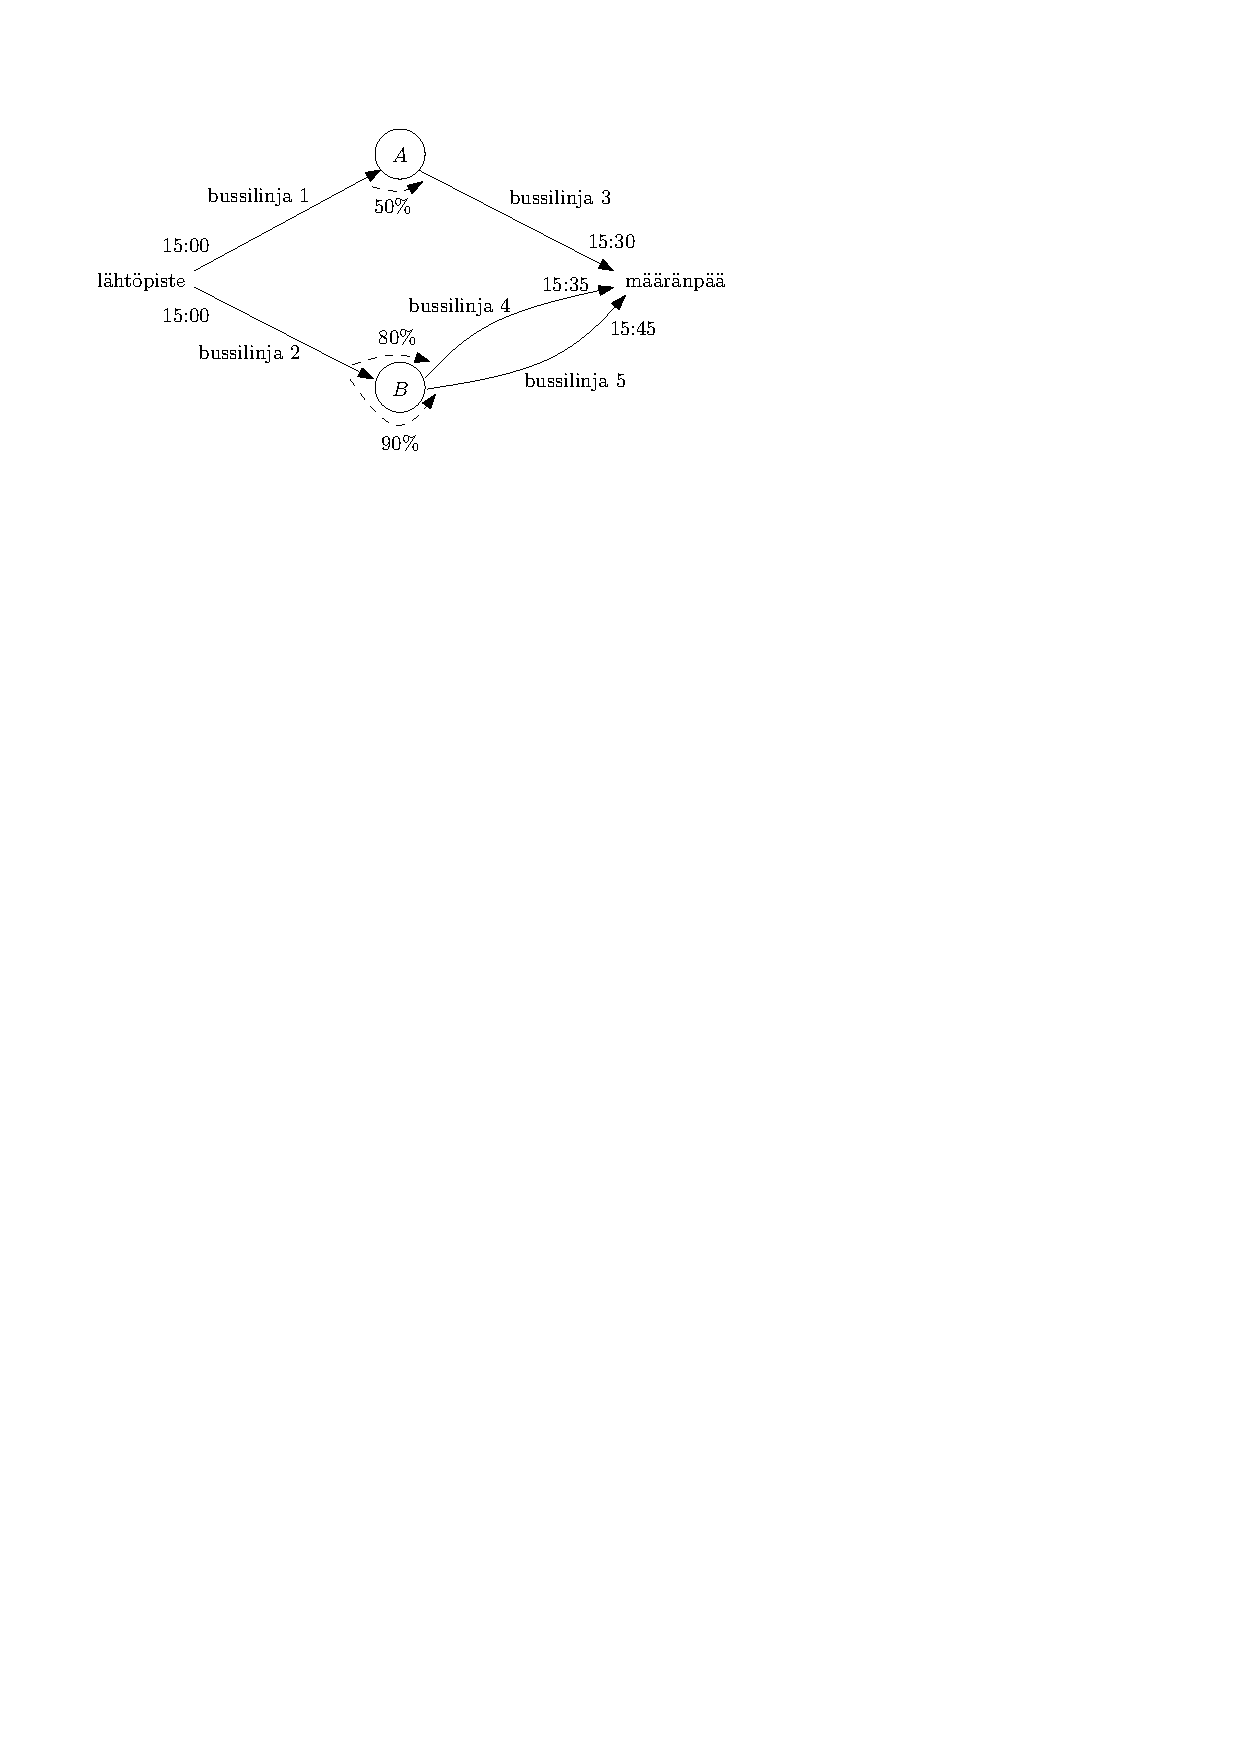
\includegraphics[scale=0.6]{matkansuunnittelu02}
%       \end{center}
%       \end{minipage}
% \end{frame} 


\subsection{Stokastinen malli}
\begin{frame}
  \frametitle{Matka-ajat stokastisessa mallissa} 
  \begin{itemize}
   \item 
    Liikennepalvelujen arvioidut ohitusajat pysäkeillä määritellään satunnaismuuttujina odotusarvojen sijaan
\end{itemize}
     \begin{center}
     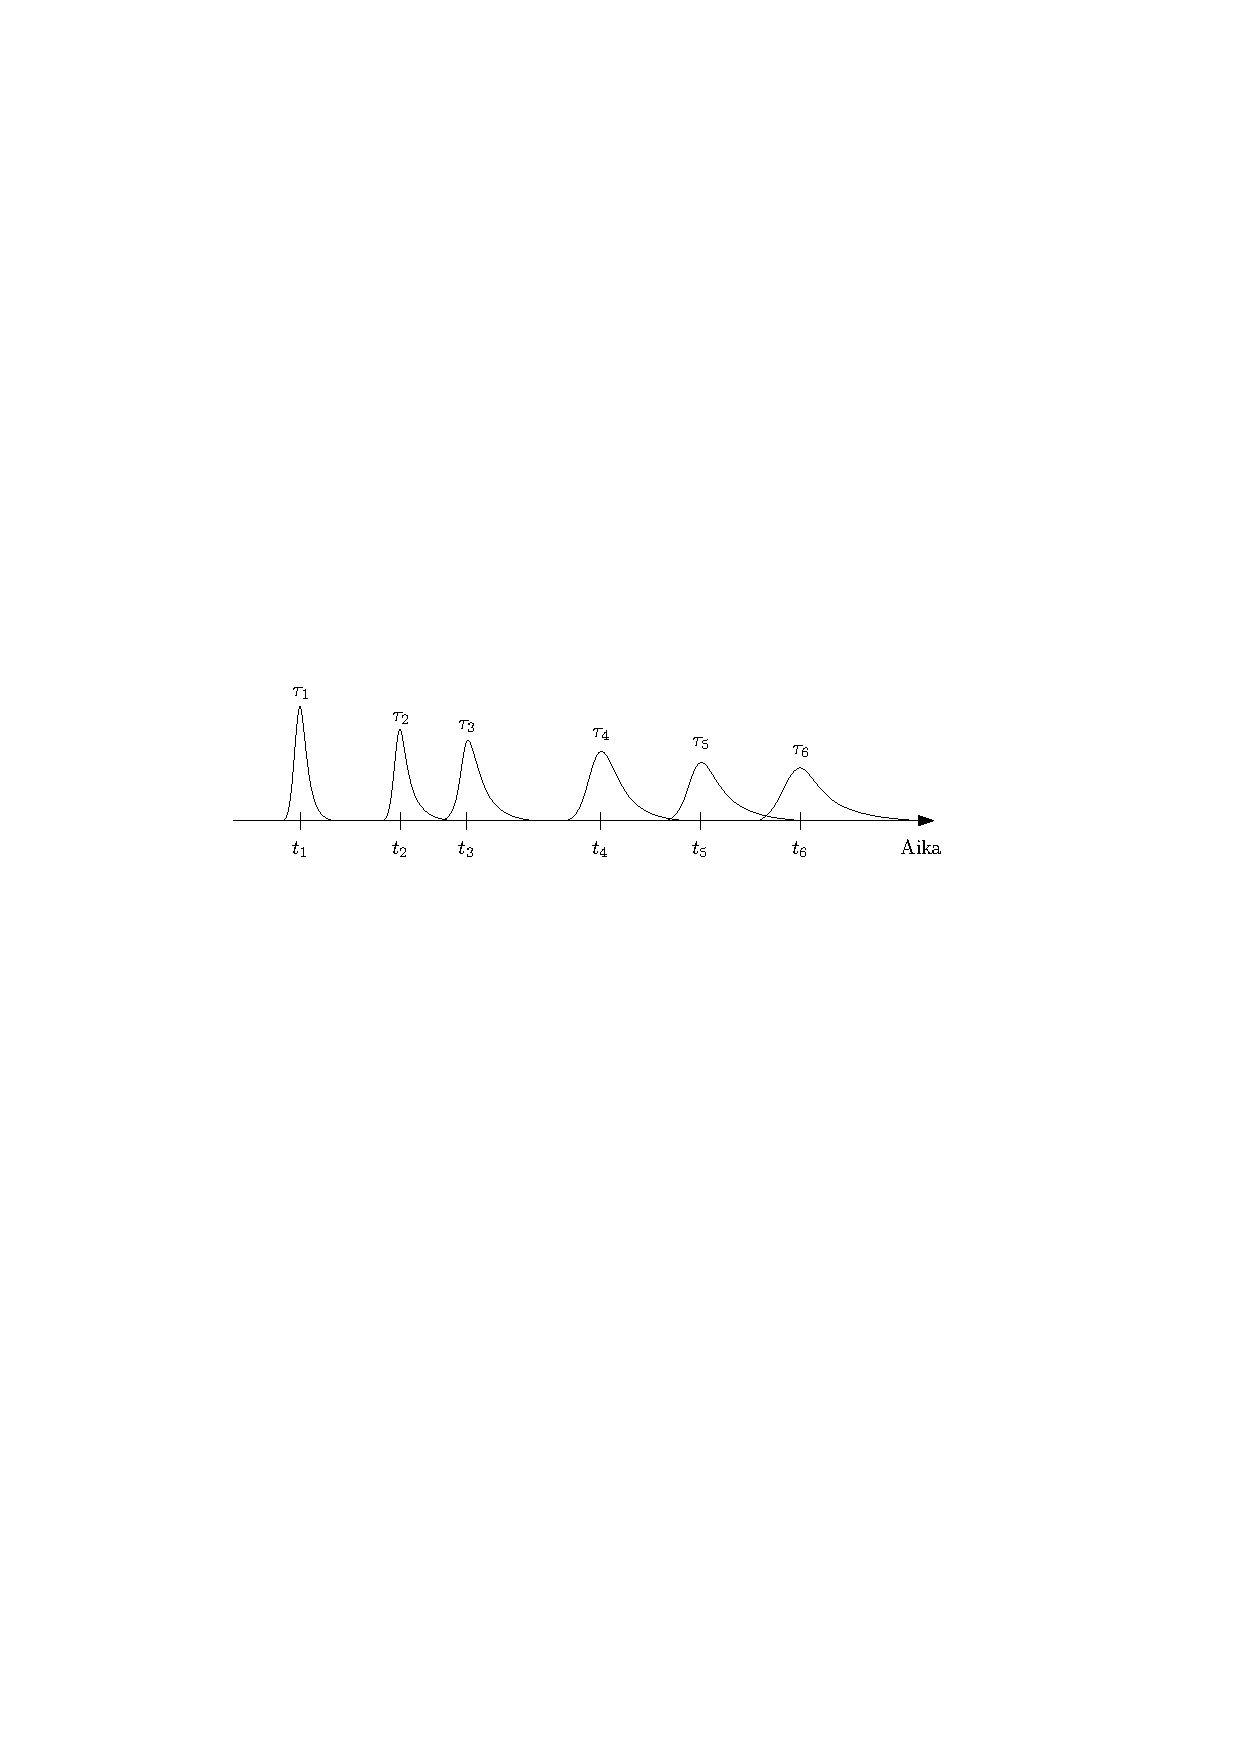
\includegraphics[scale=0.6]{stokvsdet02}
      \end{center}
\begin{itemize}
    \item
    Vaihto etapilta $i$ etapille $j$ onnistuu todennäköisyydellä $p_{ij} = P(\tau_i' \leq \tau_j)$
\end{itemize}
     \begin{center}
     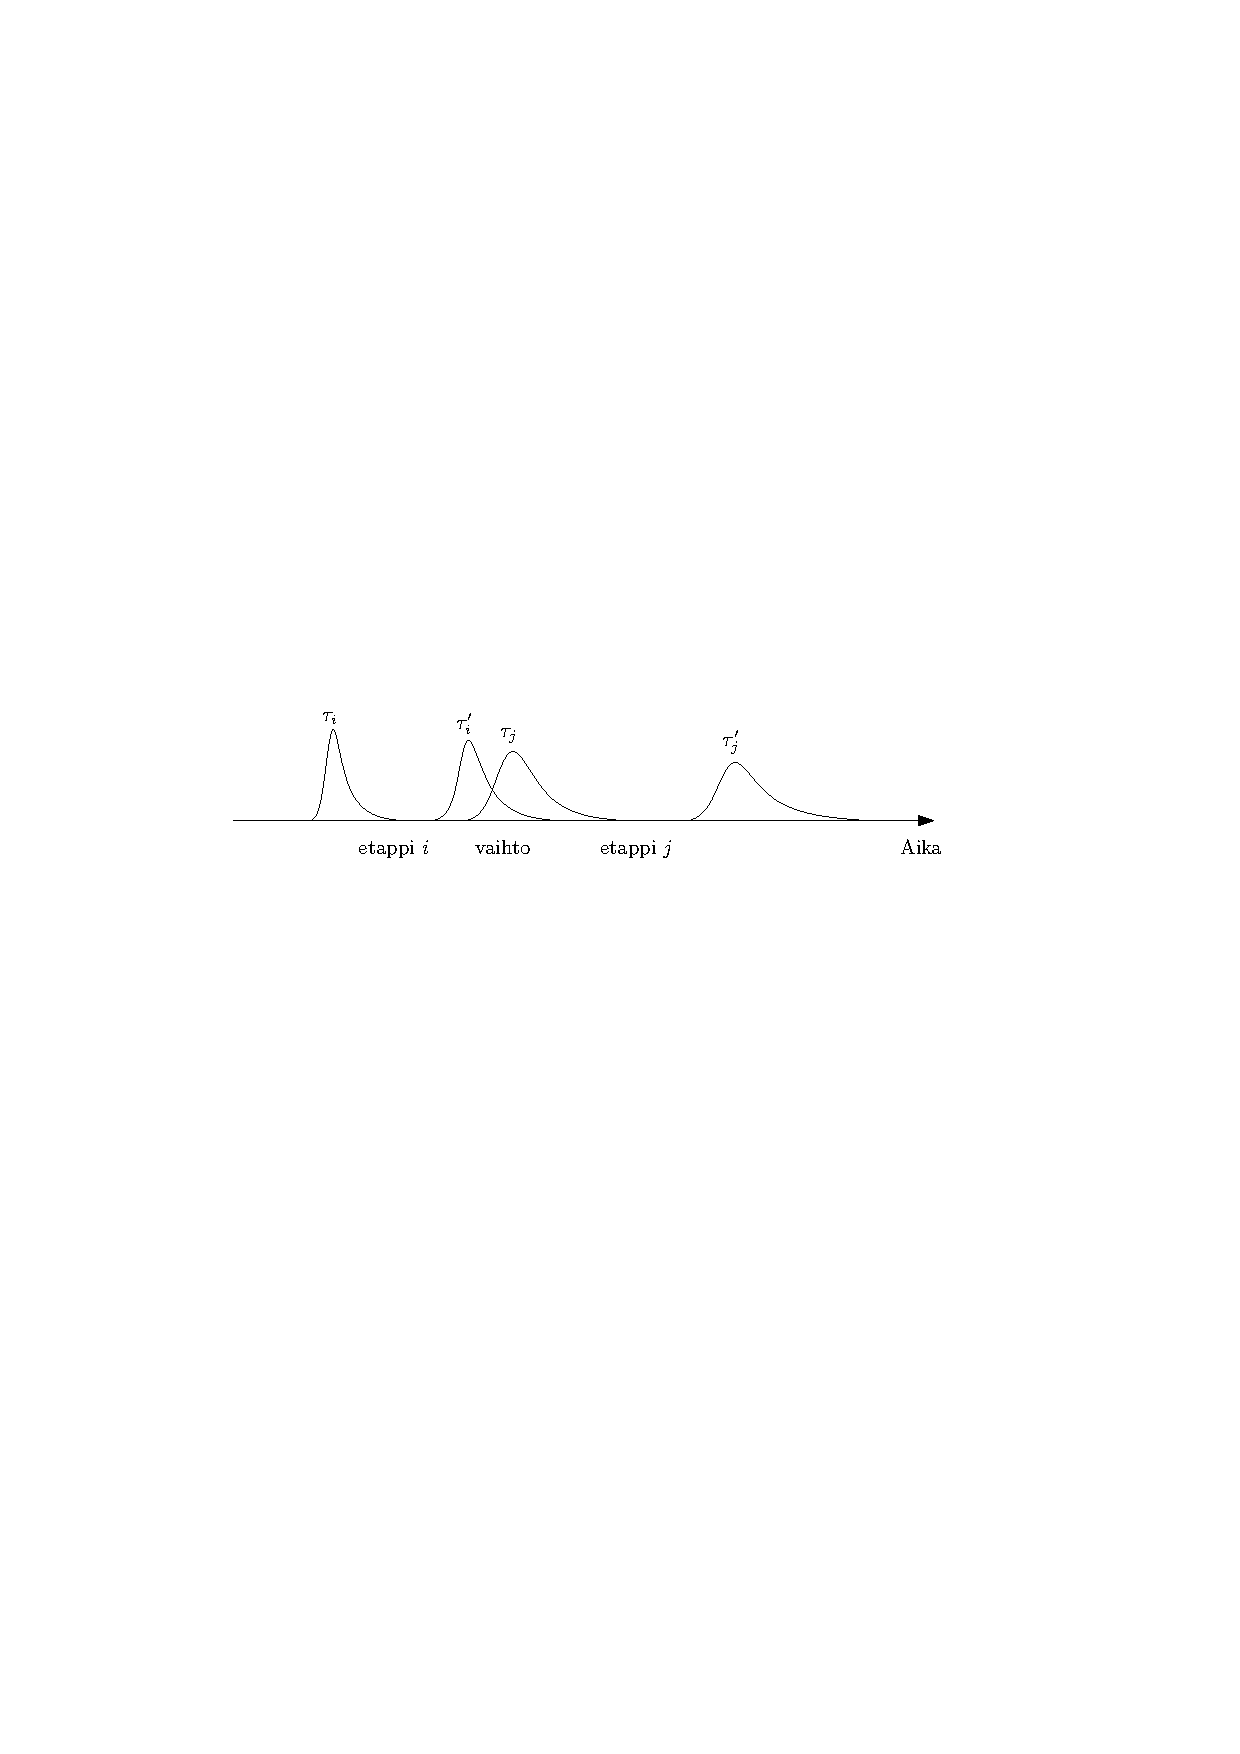
\includegraphics[scale=0.6]{transferprob02}
      \end{center}
    \end{frame} 

    
%             \begin{frame}
%   \frametitle{Todennäköisyyksien ehdollisuus matkansuunnittelussa} 
%   \begin{itemize}
%        \item
%     Onnistuneet vaihdot eivät ole riippumattomia tapahtumia
%         \begin{itemize}
%      \item 
%      Esim. Jos bussit 1 ja 2 lähtevät aikataulun mukaan samaan aikaan, on todennäköistä että 
%      vaihto onnistuu joko kumpaan tahansa tai ei kumpaankaan
%     \end{itemize}
%    \item 
%     Toteutuneet vaihdot vaikuttavat tulevien vaihtojen onnistumiseen
%     \begin{itemize}
%      \item 
%      Esim. Jos tiukka vaihto bussista 3 bussiin 4 on onnistunut, on todennäköistä että bussi 4 on ollut myöhässä
%     \end{itemize}
% \end{itemize}
%      \begin{center}
%      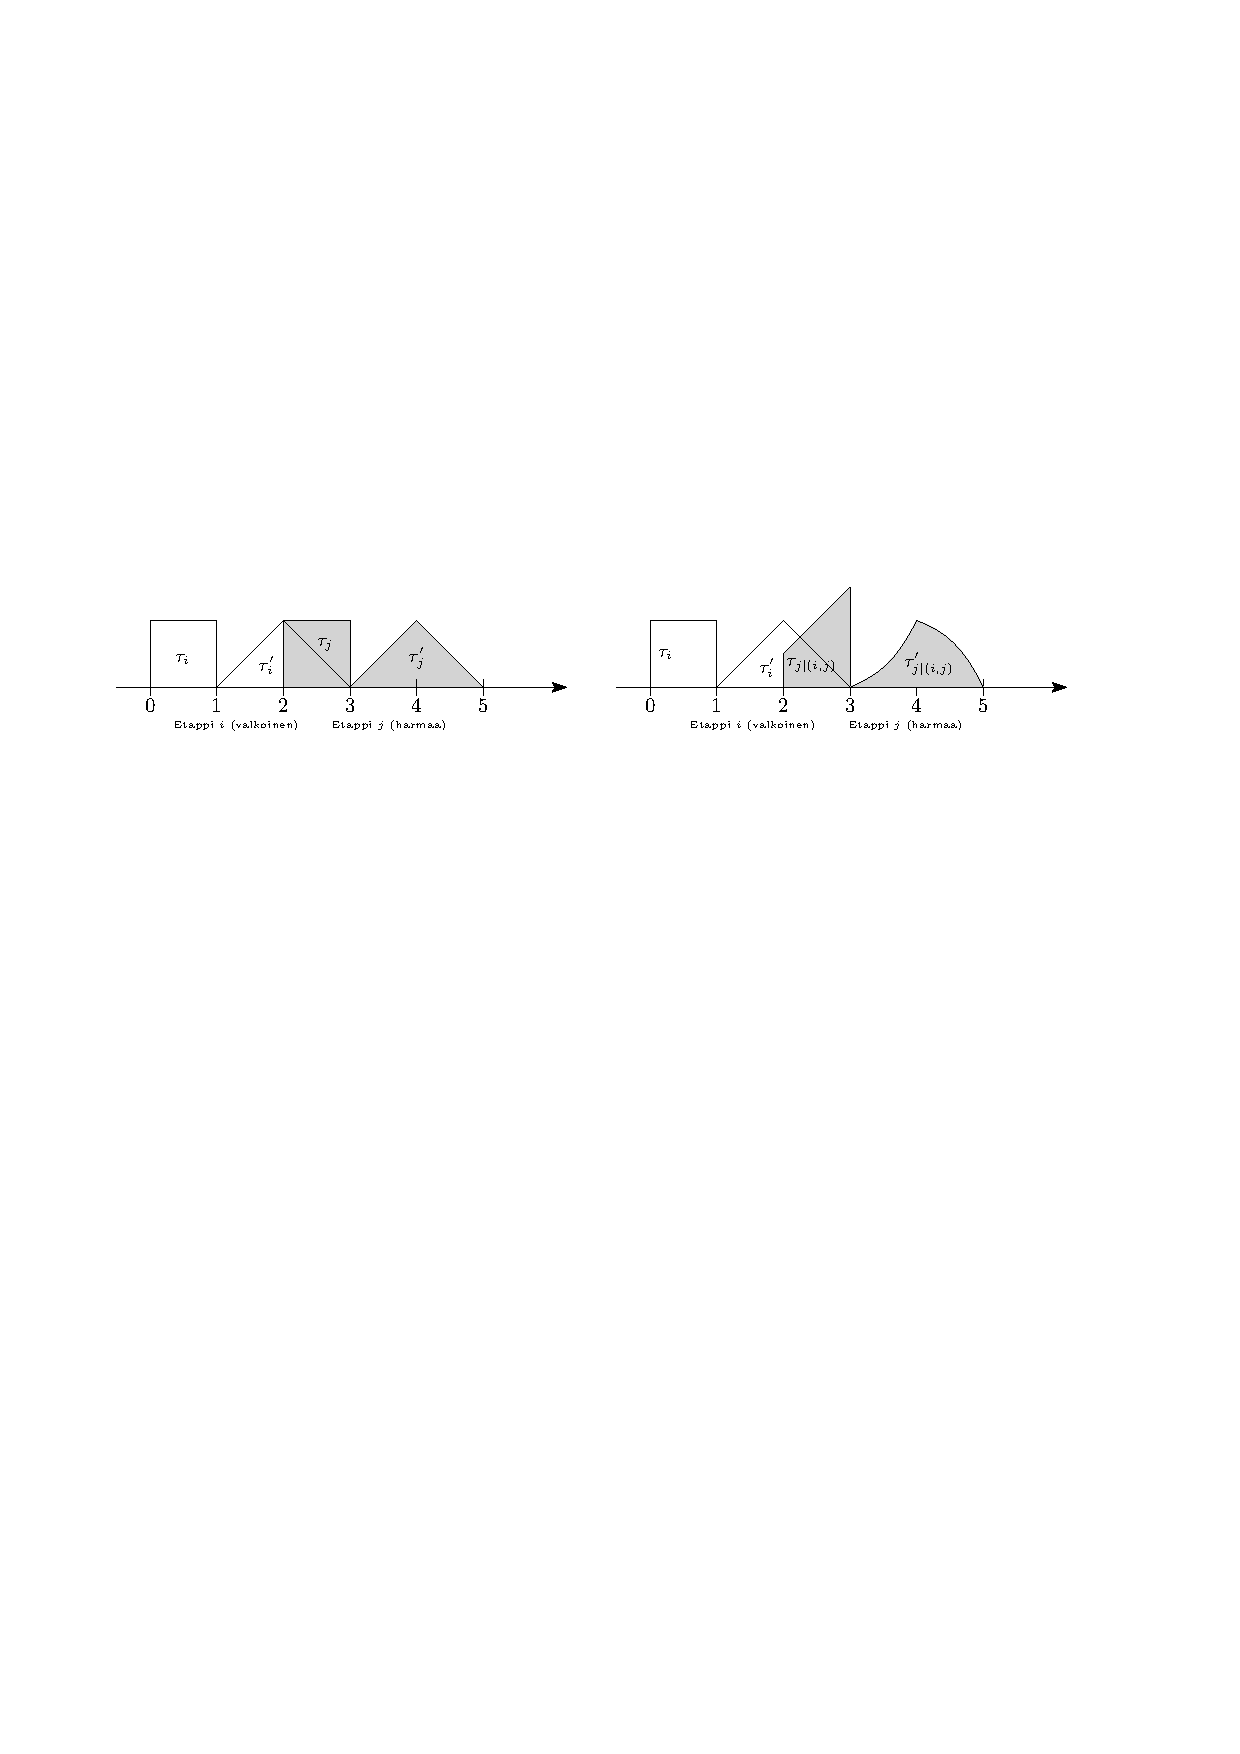
\includegraphics[scale=0.65]{stateexample}
%       \end{center}
%     \end{frame}  
%     
    
    
        \begin{frame}
  \frametitle{Markov-päätösprosessi (Markov Decision Process, MDP)} 
  \begin{itemize}
   \item 
    Matka voidaan esittää Markov-päätösprosessina etappien verkossa
    \item
    Prosessin \emph{tilat} ovat etappeja ja \emph{toiminnat} matkustajan valintoja 
    \item
    Tietty valinta tietyssä tilassa johtaa toiseen tilaan siirtymiseen
    \item
    Jokaiselle tilalle voidaan määrittää optimaalinen valinta (=matkastrategia) 
\end{itemize}
     \begin{center}
     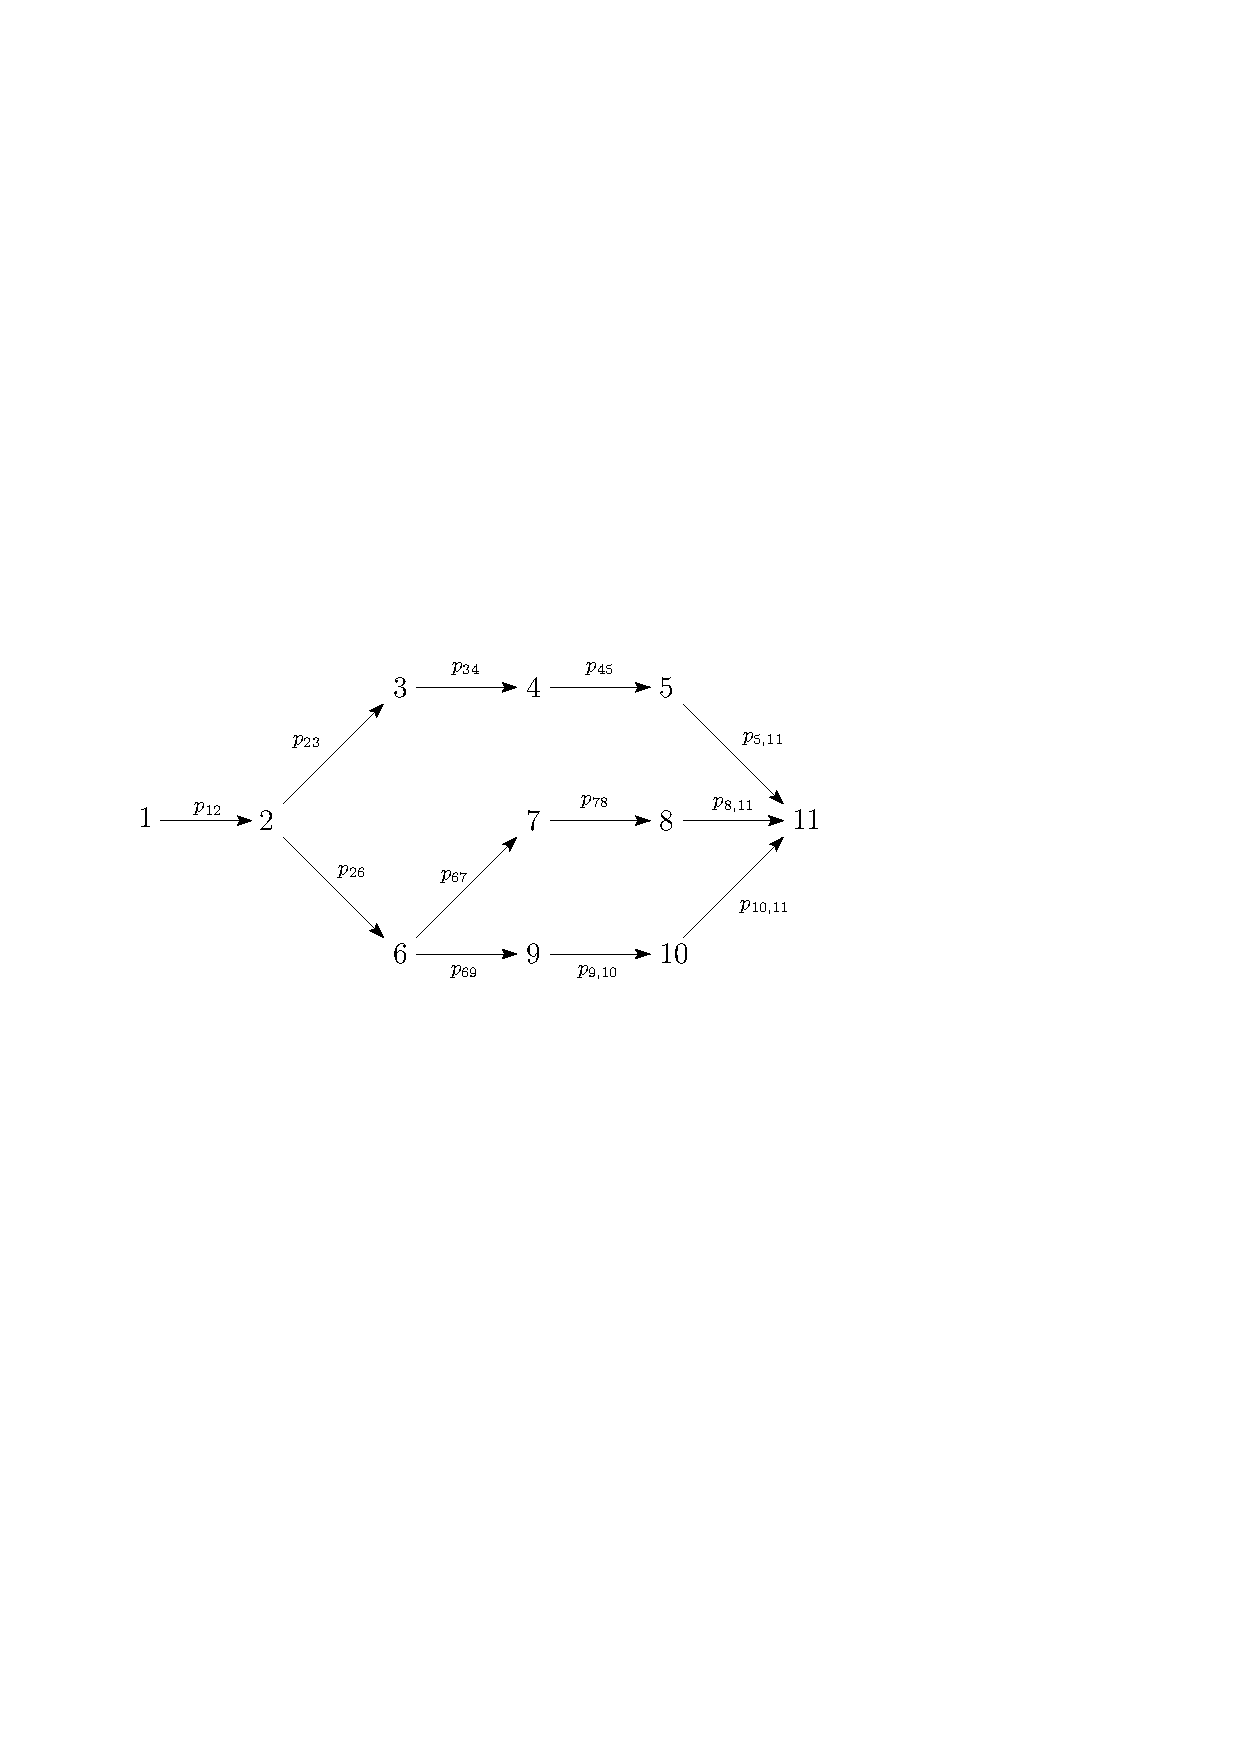
\includegraphics[scale=0.55]{walking01c}
      \end{center}
    \end{frame} 
    
    \subsection{Tuloksia}
        \begin{frame}
  \frametitle{Stokastinen matkansuunnittelu, tuloksia} 
  \begin{itemize}
   \item 
Stokastisen matkansuunnittelun merkitys korostuu kun 
\begin{itemize}
 \item 
vaihtojen lukumäärä on suuri 
\item
vaihtoihin liittyy epävarmuutta
\item
halutaan maksimoida matkan luotettavuutta
\end{itemize}
\item
Laskentaa voidaan tehostaa yksinkertaistamalla todennäköisyysmallia
\begin{itemize}
 \item 
Vaihtojen onnistumisien riippumattomuus
\item
Riippumattomuus matkahistoriasta eli aiempien vaihtojen onnistumisesta
\end{itemize}
\end{itemize}
    \end{frame}     
    
    
\section{Taloudellinen tasapaino}
\frame{\secpage}


\subsection{Yleinen tasapainoteoria}
\begin{frame}
  \frametitle{Yleinen tasapainoteoria} 
  \begin{itemize}
  \item
  Yleinen tasapainoteoria selittää kysynnän, tarjonnan, ja hintojen käyttäytymisen toistensa kanssa vuorovaikutuksessa
olevissa markkinoissa 
\item
Tasapaino = tilanne, jossa kysyntä, tarjonta ja hinta eri markkinoilla pysyvät muuttumattomina
tietyn ajanjakson sisällä.
%   \item 
%   Taloudellisessa tarkastelussa otetaan samanaikaisesti huomioon sekä matkustajien että liikennöitsijän päätökset
\item
Lähtöpaikan ja määränpään välillä on markkina
\begin{itemize}
 \item 
 Tarjonta = eri kulkumuodot
 \item
 Kysyntä riippuu kulkumuotojen laadusta ja hinnasta
 \end{itemize}
   \end{itemize}
    \end{frame}   
    

    
\subsection{Kysyntä ja tarjonta}

\begin{frame}
  \frametitle{Kysyntä}   % Insert frame title between curly braces
\begin{itemize}
 \item
Kulkumuodon kysyntä määräytyy hinnan, laadun ja vaihtoehtoisten kulkumuotojen mukaan
\item
Logit-valintamallissa kulkumuodon $i$ utiliteetti muodostuu tunnetusta osasta $V_i$ ja satunnaisesta osasta $\epsilon_i \sim \rm{Gumbel}$
\item
Todennäköisyys valinnalle $i$:
\begin{align*}
 P_i = \frac{e^{V_i}}{\sum_j e^{V_j}}
\end{align*}
%\item
%Kysyntä vaikuttaa optimaaliseen reititysstrategiaan
\end{itemize}
\end{frame}    
    


\begin{frame}
  \frametitle{Tarjonta}   % Insert frame title between curly braces
\begin{itemize}
 \item
 Kysyntäohjautuvan joukkoliikennepalvelun palvelutaso riippuu ajoneuvojen jakaumasta liikenneverkossa
 \item
 Ajoneuvojen jakauman määrittelee stokastinen reititysstrategia
 \item 
 Tilojen $r$ ja $s$ välinen siirtymätodennäköisyys $p_{rs}$ kuvaa kuinka suuri osuus ajoneuvoista
 siirtyy reitille $s$ kuljettuaan reitin $r$
\end{itemize}
\begin{center}
 %\includegraphics<1>[scale=0.65]{tilat02}
  \includegraphics<1>[scale=0.65]{tilat03}
\end{center}
\end{frame}

    
 
%     \begin{frame}
%   \frametitle{Kysyntäohjautuva joukkoliikenne stokastisena prosessina}   % Insert frame title between curly braces
% \begin{itemize}
%  \item 
%  Kysyntäohjautuvaa joukkoliikennettä voidaan kuvata stokastisena prosessina, joka muodostuu
%  \emph{tiloista} ja tilojen välisistä \emph{siirtymätodennäköisyyksistä}
%  \item
%  Ajoneuvon tila $\approx$ reitti %, kyydissä olevat matkustajat ja sovitut matkat
% \end{itemize}
% \begin{center}
%  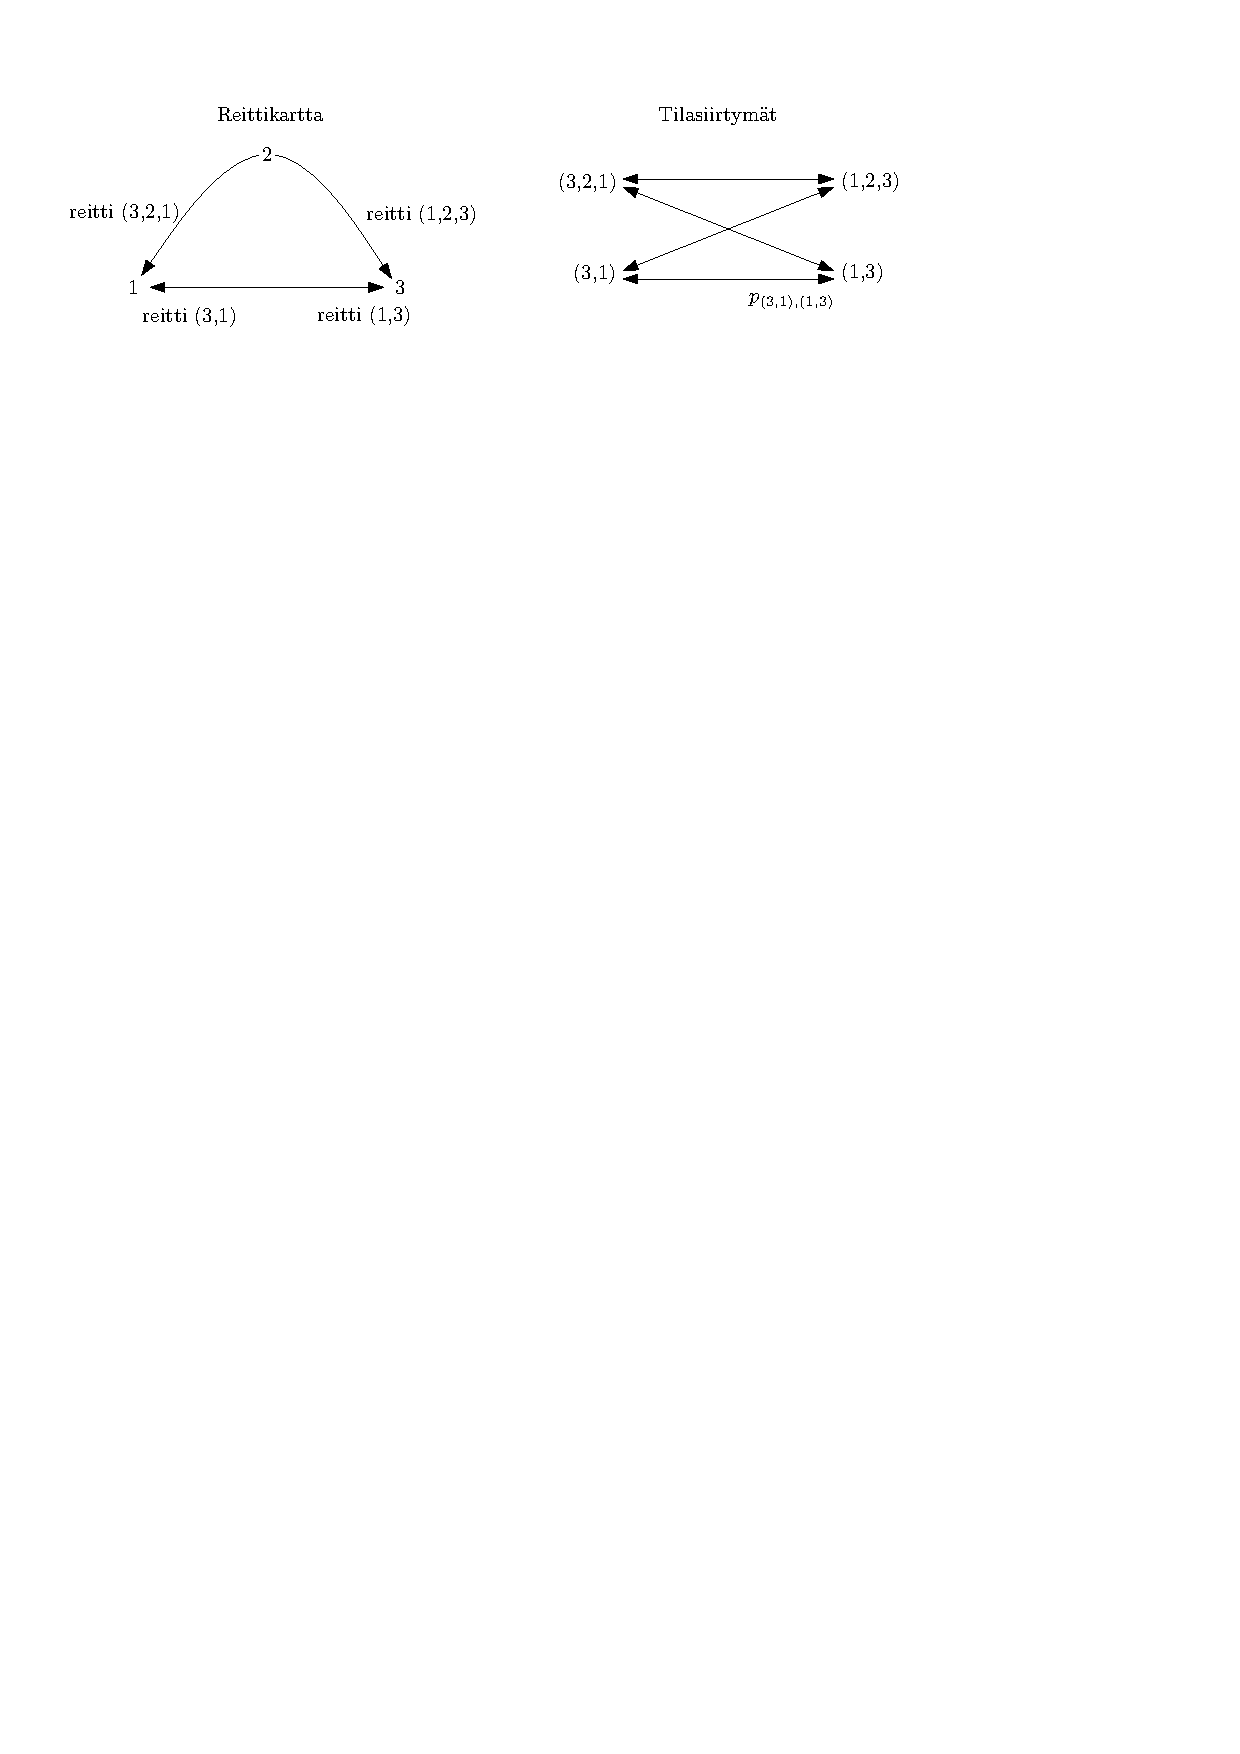
\includegraphics[scale=0.65]{tilat01}
% \end{center}
% \end{frame}


% \begin{frame}
%   \frametitle{Tilan tarkempi määritelmä}   % Insert frame title between curly braces
%   \begin{itemize}
% \item
% Tilan määrittelee
% \begin{itemize}
%  \item 
%  Reitti ja ajoneuvon sijainti reitillä
%  \item
%  Kyydissä olevien matkustajien nouto- ja toimituspisteet
%  \item
%  Sovittujen matkojen nouto- ja toimituspisteet
% \end{itemize}
% \end{itemize}
% \begin{center}
%  \includegraphics<1>[scale=0.65]{tilamaar01}
%   \includegraphics<2>[scale=0.65]{tilamaar02}
%    \includegraphics<3>[scale=0.65]{tilamaar03}
%     \includegraphics<4>[scale=0.65]{tilamaar04}
%      \includegraphics<5>[scale=0.65]{tilamaar05}
% \end{center}
% 
% \end{frame}    
    






 
% \begin{frame}
%   \frametitle{Taloudellinen optimi}   % Insert frame title between curly braces
% \begin{itemize}
% \item
% Mallin avulla voidaan optimoida ajoneuvojen lukumäärä ja matkojen hinnoittelu
% \end{itemize}
% \begin{center}
%  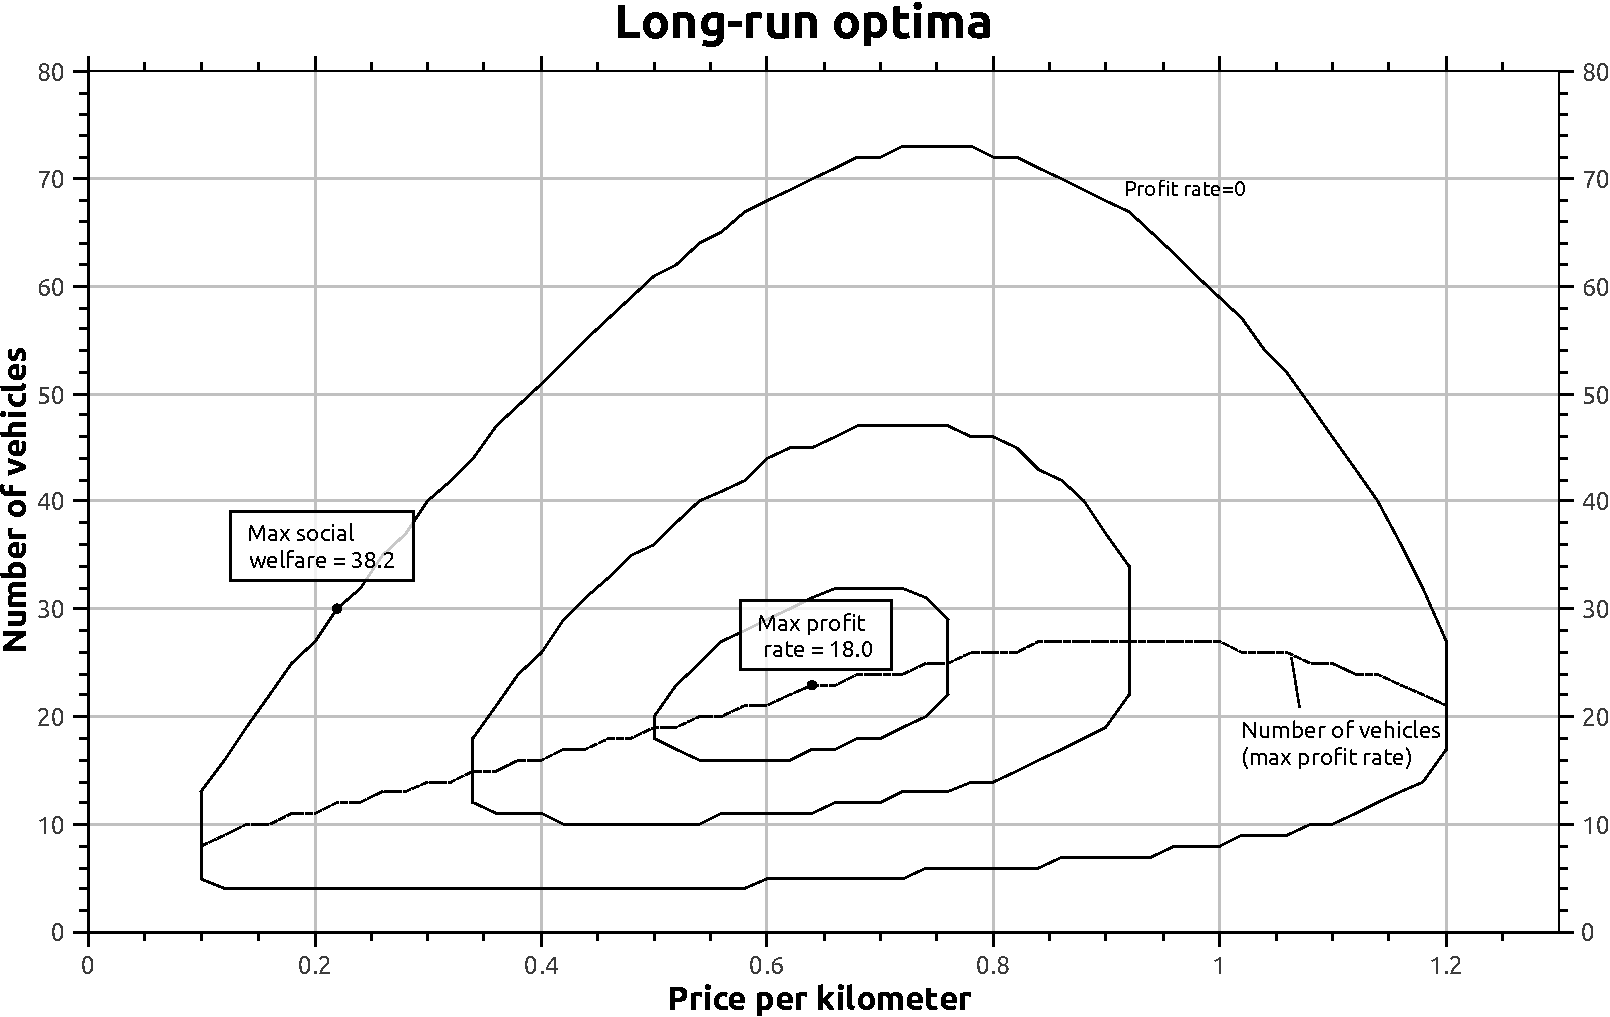
\includegraphics[scale=0.3]{a-optima02}
% \end{center}
% \end{frame}



\subsection{Tuloksia}
\begin{frame}
  \frametitle{Taloudellinen tasapaino, tuloksia}   % Insert frame title between curly braces
\begin{itemize}
\item
Analyyttinen malli, jolla voidaan kuvata kysyntäohjautuvaa joukkoliikennettä 
\item
Mikrosimulointiin verrattuna etuna on skaalautuvuus ajoneuvojen ja matkustajien lukumäärän suhteen
\item
Mallin sovelluksia:
\begin{itemize}
 \item 
Optimaalisen reititysstrategian, hinnoittelun ja ajoneuvojen lukumäärän määrittäminen eri tilanteissa
\item
Säännöstelyn vaikutusten tutkiminen 
\end{itemize}
\end{itemize}
\end{frame}

\section{Tulosten tarkastelu}
\frame{\secpage}
\begin{frame}
  \frametitle{Tulosten tarkastelu}   % Insert frame title between curly braces
\begin{itemize}
\item
Reitinlaskennassa tulee ottaa huomioon sekä kustannukset että palvelutaso: paras kokonaisratkaisu löytyy kahden optimin välistä
\item
Suuri kysyntä mahdollistaa hyvän palvelutason tuottamisen tehokkaasti
\item
Pidemmät ennakkotilausajat mahdollistavat tarkemman optimoinnin
%Kysyntäohjautuvan joukkoliikenteen pitäisi olla osa olemassaolevaa joukkoliikennejärjestelmää 
%\begin{itemize}
\end{itemize}
\end{frame}


\begin{frame}
  \frametitle{Tulosten tarkastelu}   % Insert frame title between curly braces
\begin{itemize}
 \item 
 Matkansuunnittelun avulla voidaan liittää kysyntäohjautuva palvelu olemassaolevaan joukkoliikennejärjestelmään
 \begin{itemize}
  \item 
 Vaihdolliset yhteydet (sisäiset ja kulkumuotojen väliset vaihdot), syöttöliikenne 
 %\item
 %``Liftaus'' - valmiiksi laskettujen reittien suora hyödyntäminen 
 \end{itemize}
 \end{itemize}
  \begin{center}
  \includegraphics<1>[scale=0.25]{vaihto01}
    \includegraphics<2>[scale=0.25]{vaihto02}
      \end{center}
\end{frame}


\begin{frame}
  \frametitle{Tulosten tarkastelu}   % Insert frame title between curly braces
\begin{itemize}
 \item 
Joukkoliikenteen lisäksi reitinlaskenta- ja matkansuunnittelumenetelmiä voidaan hyödyntää 
\begin{itemize}
\item
rahti- ja lentoliikenteessä
\item
lähetti- ja ruoankuljetuspalveluissa 
\item
sotilaslogistiikassa
 \end{itemize}
 \item
 Menetelmät soveltuvat erityisesti
 \begin{itemize}
  \item 
  tehtäviin, joihin liittyy rajoitusehtoja (aika, kapasiteetti)
  \item
  luotettavuuden optimointiin
 \end{itemize}
 \end{itemize}
\end{frame}



\begin{frame}
  \frametitle{Tulosten tarkastelu}   % Insert frame title between curly braces
\begin{itemize}
 \item 
Helsingin seudun liikenne käynnisti vuoden 2013 alussa kaikille avoimen kysyntäohjautuvan joukkoliikennepalvelun
\item
Enintään 60 minuutin ennakkotilausaika
\item
Useita erihintaisia matkavaihtoehtoja
\item
Toimii noin 10 kilometrin säteellä Helsingin keskustasta
\item
10 minibussia, määrää kasvatetaan
\item
Teoria on käytäntöä edellä
\begin{itemize}
 \item 
 Reitinlaskennan merkitys korostuu suurissa järjestelmissä
\end{itemize}
 \end{itemize}
\end{frame}


\bgroup
\setbeamercolor{background canvas}{bg=black}
\begin{frame}[plain]{}
\end{frame}
\egroup





% \begin{frame}
%   \frametitle{Muita tutkimusmenetelmiä}   % Insert frame title between curly braces
% \begin{itemize}
%  \item 
%  Kyselytutkimukset
%  \begin{itemize}
%  \item
% Hinnoittelu, maksuhalukkuus
%  \end{itemize}
% \item
% Mikrosimulointi
% \begin{itemize}
%  \item 
%  Algoritmien testaus
%  \item
%  Skaalaedut
% \end{itemize}
% \item
% Jonomallit
%  \end{itemize}
% \end{frame}
    
\end{document}